\documentclass[12pt]{article}

\usepackage{xcolor}
\usepackage{array}
\usepackage{makecell}
\usepackage{graphicx}
\graphicspath{ {./figures/} }
\usepackage{subcaption}
\usepackage{float}
\usepackage{longtable}

\usepackage[margin=1in,left=1.5in]{geometry}

% \usepackage{fancyhdr}


\newcommand\todo[1]{\textcolor{red}{#1}}

\def\frontmatter{%
    \pagenumbering{roman}
    \setcounter{page}{1}
    \renewcommand{\thesection}{\Roman{section}}
}%

\def\mainmatter{%
    \pagenumbering{arabic}
    \setcounter{page}{1}
    \setcounter{section}{0}
    \renewcommand{\thesection}{\arabic{section}}

    % \pagestyle{fancy}
}%

\setlength\parindent{0pt}

\author{
  Billingham, John\\
  King, Brandy\\
  LaCognata, Nicolas\\
  Simonian, Sean\\\\
  {\small Advisor: Carbone, Tom}
}

\title{Computron}

\begin{document}

\frontmatter

% Cover page with title, group number, team members, date, and any other relevant information, such as participating organizations and sponsors.
\maketitle
\newpage

\tableofcontents
\newpage

\mainmatter

% Executive summary: An administrative and technical abstract, which includes a brief description of the project, the project objectives, and the technical approach. This is page number 1.
\section{Executive Summary}
  \textit{Computron} is a computer based puzzle-solving video game that is focused
on teaching basic Computer Science concepts and the process of computational
thinking to beginners in the field. There are currently many similar resources
available, but they are either too technical for inexperienced programmers, or
 too abstract for players to apply what they learn to concepts in Computer
Science. \textit{Computron} bridges that gap by having players assemble code-like
solutions to puzzles in a simple pseudo-language. The solution is then executed
sequentially just like a computer program by an in-game character. This
execution is displayed to the player so that they can visually see the flow of
logic and adjust their solutions as needed. By beginning with the most basic
aspect of each concept and increasing the difficulty in a stepwise fashion,
\textit{Computron} is designed to help players acclimate to increasingly complex
algorithmic logic. Further, by providing feedback on solution efficiency,
\textit{Computron} also encourages players to improve upon the performance of
their solution.\\

The main objective of this project is to help individuals who are approaching
Computer Science for the first time by introducing them to basic concepts and
encouraging them to think programmatically. The layout of the game tutorial
and slow but steady increase in puzzle difficulty is specifically designed to coach
players through the concepts to ensure that they understand the basic aspects
of each concept and how to implement it in a coding environment to manipulate
data. This also supports one of the secondary objectives, which is to encourage
more people to pursue their interests in Computer Science without feeling
overwhelmed with everything that beginners typically need to learn.\\

\textit{Computron} is developed in Unity, and is playable on Windows, Mac, Linux, 
and web-based platforms. The core gameplay loop has players interact with the 
Computron Assembly Language (CAS) and a selection of datastructures to solve puzzles.
The CAS is a collection of 13 assembly-like instruction that allow players to manipulate
the elements of the puzzles they are presented. The puzzles and the 
processes needed to solve them were assembled with an eye towards basic concepts in Computer 
Science such as sorting, logical comparisons, and arithmetic. The progression of puzzle difficulty 
and the order in which each game mechanic would be introduced are based off of course outlines from
various beginner level courses, including Intro to C, and Computer Science I. Thorough research and testing has 
gone into the decisions behind these processes and defining the scope of the project.\\
\newpage

\section{Project Overview}
  \subsection{Overview}
The purpose of this project is to provide a bridge for potential computer
scientists to learn and explore the fundamentals of solving problems
computationally. Providing this insight is non-trivial, especially in
traditional teaching environments. Our approach is to present common
introductory computer science concepts in the form of puzzles and visuals in a
2D video game. This game will provide a means for those interested in
computational thinking to learn in a fun and engaging environment. The players
will not be expected to set up a development environment or learn the nuances of
specific programming languages. All of the concepts necessary to solving the
challenges should be taught to -- or discovered by -- the player through interactive
gameplay. Framing this tool as a game is an important distinction, as it allows
us to deliberately craft the players’ experience and deliver specific learning
outcomes.\\

Currently, there are many game offerings that focus on teaching computational
thinking, with most of them focusing on using “code” solutions for puzzle
solving. However, we have found that they tend to fall far on either end of a
spectrum; either the game is too abstract and the computational thinking aspect
is not well emphasized, or the game is too technical and therefore inaccessible
to beginner level programmers. It is our intention to provide a game that falls
between these two extremes on the spectrum. We want our game to teach the user
about the different commands and how they can be used to solve the puzzles
provided. This will lean away from some of the more abstract puzzle-solvers,
where the movements manipulate a character spatially instead of using the
sequence of commands to solve the puzzle. Conversely, we will use clear and
simple language coupled with visual and audio cues to explain commands and data
structures in the game, while abstracting the intricacies of language specific
commands or complex details about these elements. This will help new programmers
to more easily understand the concepts of Computer Science and use them to solve
the puzzles without requiring them to be familiar with language specific syntax
or the complexities of managing data structures in code. For example, we can
provide a heap data structure for them to use and explain its general purpose
for sorting and storing data without forcing the user to construct or maintain
the heap. Taking away the technical aspects of utilizing these elements will
allow players to focus on learning and understanding the concepts of the tools 
they are given and how to utilize those tools to solve the problem presented.


\subsection{Broader Impacts}

The audience that this game is geared towards are people with little prior
technical experience relating to Computer Science who are just beginning to
learn how to program and learn computational logic. The aim of this project is
to create an engaging platform for players to explore the process of approaching
and solving problems computationally, build a foundation for understanding the
principles of Computer Science, and prepare users for challenges they may face
in their future studies of Computer Science.\\

At UCF, the difficulties that surround new Computer Science students are easily
seen in the courses leading up to the Foundation Exam, perhaps the most obvious
with Intro to C. Students in that class are immediately faced with two major
tasks: learn to solve problems programmatically, and learn the structure and
syntax of the C programming language. Students often enter the class without 
any experience with either of these tasks, and many students end up feeling 
lost and discouraged early on.\\

Another aspect that should be considered is the unfortunate number of
underrepresented groups in STEM fields, especially Computer Science. There are
many factors that can contribute to this issue, such as individual backgrounds,
ethnicity, gender, social stigmas, disabilities, or the common lack of
preparation from underfunded public schools. Students who are already facing
pressures related to these issues may be more inclined to give up on Computer
Science when they feel lost in their first year.\\

As with any group of technically proficient individuals, it is not uncommon to
find that a number of the more experienced members inadvertently reinforce a
“gatekeeping” mindset towards STEM majors by supporting weed out classes and
survival of the fittest. This behavior can occur with upper level Computer
Science students or graduates who have seen the large number of highly
intelligent students who fail or give up on Computer Science, which could often
be avoided if better education and resources were widely available.\\

For situations like any of those described above, a resource that can provide
the tools necessary to understand and approach the concepts and challenges of
Computer Science in an effective manner would be an invaluable resource for many
individuals. Our project will provide these tools in an engaging format,
enabling players of different backgrounds and experience levels to cultivate an
intuitive understanding of computational thinking, while giving them a platform
to apply their newfound perspective to approach and solve various problems. As a
result, we hope that our game and similar resources help more students of all
backgrounds to successfully pursue their passion for Computer Science.\\

While the game strives to close the bridge between logic and syntax, by focusing
on the former it can benefit a broader scope of people, regardless of if they
plan to become software developers, or simply wish to learn the logic of
computer systems. The puzzles can act as a means to spark users’ interest in
computer science, or just to be enjoyed by a spectrum of developers and
engineers (students, industry, etc.), as the levels scale in complexity. Introducing 
a variety of puzzles that are solved using similar methods and mechanics should 
help players to begin recognizing similar patterns between different problems.\\

The game will have an engaging and easy to use interface to provide educational
value with puzzle-based challenges. The mechanics of the game will be easy to
pick up, since learning to play the game should not feel like a difficult task
on its own. The scaling of puzzle difficulty will allow the game to be welcoming
to beginners by incrementally introducing higher complexity tools and abilities
as the levels progress. By providing feedback on the basic runtime and space
complexities of working solutions, players will have the ability to learn how to
solve problems efficiently.\\

\subsection{Personal Motivations}
\subsubsection{Brandy King}
With career goals of being an Instructor of Computer Science, I was immediately
intrigued during this project proposal. As a Teaching Assistant, I have spent a
lot of time working with students in introductory level Computer Science
courses. It is often a difficult subject for students who come in with little to
no experience, and I have watched many students struggle with learning a new
programming language at the same time that they are learning to use that
language to effectively solve problems that they have been presented. I loved
the idea of an interactive game that would not only help teach people some of
the basics, but also reinforce efficient problem solving with computational
logic. I hope that the finished project we aim to provide will help students
entering computer science classes by giving them confidence in their knowledge
of concepts.\\

I am also very excited to learn new technologies, work with a team, and
experiment with game development. As it currently stands, most of my experience
with software development has been strictly course driven. Balancing full time
studies, a full-time work schedule, and a family and personal life leaves me
with extremely limited free time to pursue personal projects or devote time to
learning things outside of lectures. Working on this project will give me the
opportunity to expand my knowledge in a new programming language and to work
with a game engine. I have always been enthusiastic about video games, and I see
their value as an engaging form of media. Being able to use this platform to
convey instruction in Computer Science is a marriage of two things I am very
passionate about.

\subsubsection{John Billingham}
Coming from having no programming experience prior to college, I have seen and
experienced the disconnect between learning the correct syntax of a programming
language, and being able to think and solve problems programmatically. This game
has an aim to teach basic logic and computational thinking skills to it’s users
and I believe that this can close that specified gap that many of us have felt.

\subsubsection{Nicolas LaCognata}
I pitched this project, and I care a great deal about it. I centered my
undergraduate studies around games and simulations, and I’m excited to apply my
knowledge to create a game that is both highly engaging and educational. There
have been many occasions where my desire to pursue a career in game development
has been viewed negatively, and I’d like to be able to point to this project as
proof that the skills I have learned can provide a valuable experience to
others.\\

The idea for this project mainly came from my experience as a Teaching Assistant for Intro to
C. When I took the class, I had prior programming experience. For much of the class I
checked out mentally. I drifted through the class without really seeing what was going on.
Going back and seeing the challenges new programmers really face was a profound
experience. I want this game to help aspiring programmers, and spark interest in
our field for those on the outskirts.

\subsubsection{Sean Simonian}
Like many computer science students, I had very little programming experience
and next to zero understanding of most computer science concepts when I first
started at UCF, and I quickly found myself struggling immensely with the
introductory computer science courses. The main reason I was able to get through
the first year of computer science courses was because of friends who were
willing to help tutor me in the areas where the lectures were not effective
enough at explaining concepts to beginners. In later years, I became a much
better computer science student, and found myself in the opposite role as
before. I have had the opportunity to serve as a mentor to other students
struggling with computer science, and often tutored several people whose
professors’ teaching styles failed to meet the needs of the students. By
experiencing both sides of these situations, I have learned quite a bit about
what beginners struggle with when learning computer science concepts, and how
these concepts need to be broken down and taught in relatable ways. I am excited
about the opportunity to create a tool that can help individuals build a strong
foundation for understanding computer science.\\

Video game development was the primary reason I decided to study computer
science, which motivated me to learn to create a video game for my high school
senior project, and joined the Game Dev Knights club at UCF during my freshman
year. Later I moved away from the goal of game development in favor of interests
in software development and cyber security, so this project will provide the
opportunity to more thoroughly explore game development in a real setting with a
team without having to change the direction of my studies or career path.\\

My technical experience includes working as a software engineer for Harris
Corporation supporting programs for the Federal Aviation Administration, and
later working as a software developer for Texas Instruments supporting their
internal Data Lifecycle Management project. I have also completed a minor in
Secure Computing and Networks, have been an active member of UCF’s Collegiate
Cyber Defense Club for the past few years, and am currently part of the
operations team for Hack@UCF to support the club. Each of these experiences has
helped me build various skills that should be useful for this project. Working
on this game will provide the opportunity to develop additional skills in areas
where I would otherwise be lacking.


\newpage

\section{Legal, Ethical, and Privacy Issues}
  Since this project will hopefully have real-world impacts, there are a number of
potential issues and precautions to address from the beginning. The fact that
this project is not sponsored, and is not expected to generate any revenue
directly or indirectly, suggests fewer potential legal issues than sponsored
projects or projects that would provide a company with monetary gain. We have to
be careful of potential copyright infringement, since creating a game that is
very similar to existing games could introduce legal issues. If we use any
publicly available game assets, then we will have to ensure that we are
compliant with any terms of use. We plan on using original artwork for the game,
and the art will have to be royalty free, along with all other game assets.
Another legal consideration is the fact that members of our group have had to
sign non-disclosure agreements with multiple large companies relating to past
employment, but this is not expected to cause any issues at this time.\\

Ethical considerations must be made for our game and the testing we perform for
development. In order to optimize the educational capabilities of the game, we
are conducting tests on as many unaffiliated individuals as we can throughout
the development process. When performing any psychological tests, it is
important to create a controlled environment. Participants should be given a
waiver to sign before they participate in a study. For the sake of simplifying
the process and minimizing liability, we will not be performing these tests on
minors, nor will we include minors in our target audience. Since the target
audience for our game is people with little to no experience learning computer
science and computational thinking (primarily around the college freshman
level), we are able to set the target age at over 18, while also expecting that
the game would be useful for a number of younger students in the middle and high
school range.\\

Our team strongly supports the universal right to privacy for all people, and
our product will reflect that. No personally identifiable information will be
intentionally collected or stored about users. If our project includes a web
component and/or remote database, all data should be encrypted while in transit
or at rest. If we need to create user accounts and/or collect user’s email
addresses for scalability to verify user accounts, then those will have to be
encrypted and stored securely.

\newpage

\section{Requirements}
  \subsection{Functional Requirements}
\begin{enumerate}
	\item Be a playable video game
	\item Help users learn and understand foundational computer science 
		concepts
	\item Have an easy to use 2D interface to encourage beginners
	\item Present the user with various challenges and puzzles to solve
	\item Provide beginner level explanations to concepts as they’re introduced
	\item Display visuals to help users understand concepts that are being introduced
	\item Encourage user to apply concepts to solve subsequent challenges once it has
		been introduced
	\item Supply hints to user when requested
	\item Allow user to see their previous solution attempts for a level
	\item Simulate the execution of player’s solutions with animated visuals
		corresponding to the steps
	\item Inform player of the accuracy and efficiency of their solution
	\item Give generalized feedback on the effifciency and space complexity of a solution
	\item Permit user to speed up the simulations
	\item Halt solution simulation in the case of:
		\begin{itemize}
		\item Incorrect Output
		\item Runtime Error
		\end{itemize}
	\item Support scalability so additional levels can be added later on
	\item Interface will be suitable for users with certain common disabilities:
		\begin{itemize}
		\item Color blindness
		\item Deafness
		\item Epilepsy
		\item Auditory stimuli sensitivities
		\end{itemize}
\end{enumerate}

\subsection{Non-Functional Requirements}
\begin{enumerate}
	\item Demonstrate concepts visually with 2D animations simulating the 
		execution of a user’s solution to a challenge
	\item Allow user to select levels
	\item Design a simple pseudo-language with restricted capabilities for the
		user to solve challenges
	\item Interpret the set of commands in a user’s solution
	\item Solutions must follow interpreter requirements in order to be simulated
		(similar to compile time errors)
	\item Simulation will detect errors and halt immediately if an error
		is encountered (similar to runtime errors)
	\item Store user’s solution attempts for a level
	\item Evaluate the space complexity of a solution by tracking the data
		structures used
	\item Interface will accommodate users with certain common disabilities:
		\begin{itemize}
		\item Components in which color is significant to gameplay will use 
			a colorblind friendly palette
		\item Components in which sound is significant to gameplay will have
			corresponding text and/or visual indicators to accommodate deaf users
		\item Avoid presenting bright flashing colors/lights that may trigger
			epileptic users
		\item Avoid sudden loud or unpleasant sounds that may disturb users with
			auditory sensitivities
		\end{itemize}
	\item Run on Windows and Mac computers, as well as Linux subsystems
	\item Perform smoothly on standard hardware
	\item Present efficiency metrics to the player after they successfully 
		solve a puzzle
	\item Personally identifiable information about users will not be collected or stored
\end{enumerate}
\newpage

\section{Game Design}
  As a student sponsored project, we were faced with some very unique
challenges. As a team we had to answer some very important questions:

\begin{itemize}
    \item What exactly is the problem we wish to solve?
    \item What is our solution to this problem?
\end{itemize}

We quickly recognized that finding good answers to these questions was imperative to the success of our project.
This section of the document will discuss our efforts in answering these fundamental questions.

\subsection{Ideas}
  The beginning of our project was characterized by a great deal of brainstorming. We took great strides
to avoid a herd mentality when discussing possible game mechanics, themes, and designs. We frequently
separated to come up with ideas as individuals before returning to blend those ideas together into a more
cohesive whole.

\subsubsection{John Billingham}
\paragraph{Abstracting Conditional Jumps:} ~\\
Conditional jumps run the possibility of bringing complex logic that may overwhelm
or confuse the player. While our instruction set is similar to assembly, we would like
to minimize the complexity that is associated with assembly logic. One way that traditional
higher level programming languages achieve this is by introducing nested if/else conditional
statements.\\

These are essentially the same thing as a conditional jump. A statement is evaluated to
true or false and the flow of logic (the next instruction to be executed and those after)
depends on this produced boolean value. Nested if/else blocks make this flow of logic
far more visually appealing. We must be careful though, by not allowing the player to create
additional complexities with confusing nested logic. Limiting the number of conditional
instructions that the player has access to can solve this problem. We can also just blatantly
limit the number of nests that we allow with conditional logic. It is important that we
do not create more complexities while trying to remove some here.\\

\paragraph{Jump Instructions as a Resource:} ~\\
Distributing jump instructions as a finite resource can enforce the idea of runtime
efficiency for those who play the game. The more jumps a player uses, especially those
that are not necessarily needed, the more it may slow down a player's solution. A puzzle level may
be able to be solved in ten different ways, but maybe there is a solution that is the fastest
and most efficient in terms of runtime and space.\\

We can push players towards the efficient solution by distributing jump instructions scarcely.
A reward system could also be introduced as a means to enforce these concepts. Players with
faster solutions (fewer steps/instructions executed) could gain some sort of point based
score that maybe allows them to unlock more levels down the road.\\

\paragraph{Data Structures:} ~\\
Our initial inspirations and ideas for this game only contain one data structure that is
used on the game board: registers. Items can be placed in and taken out of these registers and that
is it. Registers support two basic functionalities:
\begin{itemize}
	\item Item goes into register
	\item Item goes out of register
\end{itemize}

Computer Science relies on many other equally important data structures like stacks,
queues, and heaps. Rather than use just registers as components that players can use on
the game board to solve a puzzle, we can bring in other structures that allow them to
optimize their solution even further. This would really drive in some core Computer Science
material, something that most educational games of this genre fail to do.\\

These data structures were specifically mentioned because they also
all support two main functionalities like the registers above.\\

Stacks:
\begin{itemize}
  \item Push
  \item Pop
\end{itemize}

Queues:
\begin{itemize}
  \item Enqueue
  \item Dequeue
\end{itemize}

Heaps:
\begin{itemize}
  \item Insert
  \item Delete
\end{itemize}

Limiting data structures to these same input/output type of mechanisms allows our
Actor to easily interact and communicate with these new game components.\\

Puzzle levels that were solved using a naive solution earlier on may be able to be
optimized at a later date after certain data structures have been introduced. We can
structure our puzzle level progression system to take this into account.\\

\paragraph{Atomic Move instructions:} ~\\
Having the Actor pick up an item and place it down as two separate instructions
makes our instruction set feel too much like assembly code. Replacing this with one
atomic move instruction abstracts these two commands, making it simpler for the player
to understand its use.\\

The previous functionality is preserved but the steps that a player has to take to achieve
it is reduced. This should help players solve levels faster by removing an unneeded
intermediate step of work.\\

The move instruction would contain two parameters: a source and a destination. When the
instruction is executed, the Actor moves to the source, picks up the data located there, and moves
it to the destination specified by the instruction. This also makes our instruction set seem
more like orders for our Actor to follow rather than a straight controlling of the Actor's
every move.\\

\paragraph{Add/Subtract specificities:} ~\\
Add and subtract instructions would work very similarly to the move instruction
mentioned above. Two source registers would be specified, either to be summed or differenced,
as well as a destination, where the sum or difference is placed.\\

The Actor does the animation work of adding or subtracting data and moving it to the correct
location. This again removes additional logic that the player has to think through when
solving a puzzle.\\

\paragraph{Color-based indexing system:} ~\\
The player accesses instructions through a color-based indexing system.
Colors represent specific data structures on the game board, while indices represent
specific locations within a colored data structure. ``Green sub 3" would indicate the
third index within the green data structure.\\

This is meant to give the player more control over the locations that exist on the
game board. It is also meant to drive Computer Science concepts of indexing and accessing
different places in memory. We would conventionally use a variable and an index to access
certain data structures, but the variable is replaced by a uniquely colored visualization
of a data structure.\\

\paragraph{Return instruction:} ~\\
Allow the user to choose a data structure to return as their output. The
contents of the data structure are checked against the expected output for the
puzzle level. The player chooses the data structure they wish to return by choosing
that data structure's color in the output game object.\\

\paragraph{Debugging levels:} ~\\
The player can step back and forth through their solution, one instruction at a time,
and the Actor should support these operations to show a visual debugging process. This
visual control can help players find problems within their solution, allowing them to
progressively reach the end of the puzzle level.\\

\paragraph{Broken solution given initially:} ~\\
A proposed puzzle type where the player must fix a broken solution that is given when the level starts.
This can be used in conjunction with tutorials to teach new concepts. This enforces the functionality
of certain data structures by having the player interact with a broken data structure being
introduced to them.\\

If a player has messed with and fixed a broken data structure prior to using it in one of
their future solutions, our hope is that their ability to use this data structure and think in
terms of this data structure when building a solution will be increased.\\

\subsubsection{Brandy King}
Many of my ideas for Computron came from observing players struggle with games like \textit{Human
Resource Machine} and \textit{7 Billion Humans}. I focused a lot on the shortcomings of those games; 
more specifically, I aimed to fill in what they were lacking in terms of the accessibility that they provide 
to inexperienced programmers. Additionally, I wanted the game to feel engaging and rewarding for 
players, something that is often overlooked in the development of educationally focused video games. \\

\paragraph{Declaring Variables and Data Structures:} ~\\
When we were discussing the scope of the instruction set we wanted for our game, I put forward the idea
of including a ``declare" instruction that players would use to initialize a variable or data structure for use
in their solution. This would be tied dynamically to the instructions they are able to use, as some instructions
are only applicable to these items, like the Move and Copy commands. These commands have a blank field
that the user has to fill with an available structure, so if they didn't declare the item, they wouldn't be able to
link it to the command.\\

The hope was that this would reinforce the notion of instantiation of data structures for use in a program. By
making the player responsible for managing the data structures, it would emphasize how a programmer
is responsible for declaring and utilizing variables and data structures to handle data within an algorithm. In
discussing the mechanics of how this would work, it became clear that implementing the declaring functionality
as a command would be very difficult to do dynamically, so it was adapted to be its own section, separate from
the solution that the player builds. This way, the variables and data structures could still be handled dynamically --
both in their declaration and in their attachment to instructions in the solution.\\

\paragraph{Tutorial Levels:} ~\\
It became clear very early on that many of the current game offerings in this arena did a lackluster job of
providing a solid introduction to their game. Many of the games escalated in difficulty far too quickly for
players new to programming to follow along with. They could complete the first few introductory puzzles,
but were quickly lost when the game mechanics became more complex or increased in scope. It was evident
that having a very solid tutorial aspect to our game was vital to our success in conveying concepts.\\

I proposed that we intersperse tutorial levels between puzzles in the flow of the game. We already knew that
as players progressed through the game they would unlock access to new data structures and commands. As
soon as a new item was unlocked, a tutorial level would be the next puzzle in the game. This would be a free-play
level with unlimited input and no determined solution wherein the player could experiment with and explore
the functionality of their newly unlocked item without the pressure of immediately needing it to solve a puzzle.\\

In order to ``complete" each tutorial level, the player would be required to complete a short to-do list that
covered the basic concepts of their new command or data structure after reading a brief description of the function
and mechanics of what that item does. For example, a Heap tutorial level to-do list would include:
\begin{itemize}
	\item Declare a Heap
	\item Put five inputs in the Heap
	\item Remove five inputs from the Heap
\end{itemize}
As each item on the to-do list is completed, it will be checked off automatically for the player. Once it is fully
completed, they can elect to exit the tutorial whenever they are ready and move forward to the next
puzzle, which will necessarily utilize the new element in its solution. \\

\paragraph{Limiting Certain Commands:} ~\\
By limiting the capabilities of certain commands, we can better communicate to players the functions of certain
elements in the game. As previously stated, the Move and Copy commands are only useful in conjunction with a
variable or data structure. These commands could be in the list of available instructions for a level, but they would be
dulled out and inaccessible to the user until a proper variable or data structure was declared.\\

Similarly, some commands will not be able to be used with certain data structures. For instance, the Add and Subtract
commands can be used on variables, but we should not allow players to arbitrarily use Add or Subtract on the
top element of a Heap, Stack, or Queue. The player would be required to remove that element from the structure,
manipulate the data, and then put the modified data into the structure. This reinforces the core concepts of how
these structures are used for storage, and will also encourage players to select the right type of structure depending
on how they may need to manipulate the data in that level.\\

\paragraph{Instruction ``Jumbotron":} ~\\
In \textit{Human Resource Machine}, as the character is acting out the instructions for the player, there is an indicator
in the panel containing the player's solution that points to which command is being executed at that time. While this
is very useful when trying to trace through a solution or debug a problem in the code, it is also a bit too subtle
and most users that I observed didn't notice it at all, even when they were stepping through their solution one
command at a time.\\

From this, I got the idea of introducing a ``Jumbotron" element in the User Interface of the puzzle that would
show up during execution and broadcast which instruction was being executed at that time. My hope was that the
text of the command the user had in their solution paired with the actions of the Actor on the screen would more
directly emphasize what action was caused by each instruction. This would, in turn, create an association between
the commands and the way they effect the flow of the puzzle, which was something that seemed to be lost to new users
who were inexperienced at programming.\\

\paragraph{Indentation Within Conditional Blocks:} ~\\
When conditional statements are presented in the games we playtested, there was no indication of which code
belonged inside of the conditional block or where that block ended. This is because the conditions had to be
controlled with jump statements. However, for users who are not accustomed to scoping and how code blocks
work, it is very unclear where exactly a jump statement should go to end a block of code, or even to use a jump
statement in the first place.\\

Using indentation within conditional blocks provides a much clearer picture to the user of exactly what code belongs
to which piece of the logic in their solution. This is seen consistently throughout real world programming and coding
syntax, where indentation and spacing are paramount to the readability of code. By adopting this convention
in our pseudo-language, we can not only set up players for the way real programming languages are laid out, but
also communicate to them more clearly the flow of their solution.\\

\paragraph{Points-Based Scoring of Solutions:} ~\\
Making an educational game that people enjoy playing is extremely challenging. It is very important that, in addition
to being instructive, our game should also be enjoyable. We can foster an early love for Computer Science by
creating a game that players want to return to. This can be achieved by implementing game mechanics that the
player can reference to see how well they are doing, and that invite the player to continue practicing their solutions.\\

A point-based scoring system is a popular device implemented by many games. Scoring a solution out of three stars,
for example, clearly indicates to a player how well they solved the puzzle and whether or not there is room for
improvement. Simple mechanics like this can be a strong motivator for players to return to previously solved levels
and try a different approach in an attempt to get a better score. Encouraging this second look at a solution will
stimulate the idea of reevaluating old code and making an effort to improve upon it, especially once new concepts
have been learned.\\

\paragraph{Individual Puzzle Solutions Connecting to Solve Larger Puzzles:} ~\\
This idea is borrowed from the game \textit{SpaceChem}, which is a game that implements computational thinking
to solve puzzles. It falls more on the abstract side of the spectrum, but it has a game mechanic where the solution to
several puzzles is combined together as the input for another puzzle down the line.\\

In relation to our game, my idea was to have individual puzzles be part of a larger puzzle. The efficiency of each
of the solutions to three smaller puzzles will dictate how well each of those pieces works together, and ultimately
how well the puzzle that relies on those three pieces can be solved. This could be effectively implemented through
an overall game theme where each puzzle makes sense to be one component of a larger piece. This idea of nested
reliance will reinforce motivating players to revisit puzzles that they have already solved to find more efficient solutions,
which can in turn lead to a better solution overall.\\

\subsubsection{Nicolas LaCognata}
My biggest inspiration for this project was \textit{Human Resource Machine} by the Tomorrow Corporation.
\textit{Human Resource Machine} is a charming little puzzle game that tackles the problem we settled on solving,
the gamification of computational thinking. I love the game and find it highly engaging. However, playtests
with non-programmers clearly demonstrated the games' shortcomings when dealing with its target audience.

\paragraph{Basic Mechanics:} ~\\
When brainstorming the basic mechanics of our game, my mind continually strayed towards \textit{Human Resource Machine}.
Through playing the game, and watching others play it, it became clear that Tomorrow Corporation's decision to stick with
an assembly-like instruction set was an extremely effective mechanic.\\

The assembly like instructions were simple enough for non-programmers to understand, and easy to compose 
together to make more advanced puzzles and solutions. Even at the risk of having our game appear as a rip-off, 
I thought it would be wise to adapt these mechanics.\\

\paragraph{Data Structures:} ~\\
After surveying many games in the problem space, we failed to find an example of a game that tackles computational thinking
with the aid of Data Structures. Data Structures are such a fundamental part of being a programmer, that their omission in these
games seemed incorrect.\\

\paragraph{Card Game Mechanics:} ~\\
During our prototyping sessions, I came up with the idea of “Memory Cards”.
These memory cards would allow the player to declare register locations and data
structures before their program starts running. Making the mechanics of placing these
memory cards similar to a game like \textit{Hearthstone: Heroes of Warcraft} would be
a natural and compelling addition to our puzzle format. This “Memory Card” interface
would be separate from the normal instruction writing interface, which helps reinforce
the idea that they are separate parts of the puzzle. \\

Another benefit of this design is the ability to deliver new instructions and data structures
to the player in a familiar (and exceptionally game like) way, card packs. Card games deliver
goodies to players in little packages whose contents appear hidden. While discussing adapting
card game mechanics, we realized that having that little unboxing moment when introducing new
instructions to the player could be highly compelling. Other games in our problem space often
silently drop new instructions on the player as they progress. By making the new instructions
appear as a reward, we can ensure that the new mechanic being introduced gets the appropriate
attention from the player. \\

\subsubsection{Sean Simonian}
Much of my inspiration for creating this game comes from my experiences of being in the positions 
of struggling greatly with introductory computer science concepts, to later tutoring beginner 
Computer Science students. Considering common issues that beginners struggle with, as well as 
feedback and observations from non-technical students playtesting our game prototypes, serves 
as the strongest indicator of how we need to design our product in order to best serve our target 
audience. Like the other team members, I drew inspiration from a few games that share similar goals 
or mechanics as what we envisioned for our game, such as \textit{Human Resource Machine}. As 
someone with less fondness and experience with the video game industry, I also spent some time 
focusing on the broader idea of creating a tool to benefit students learning Computer Science concepts,
 and I explored ways to pivot the basis for how we could create such a tool. Having real-world 
experience and passion for both software development and cyber security has greatly influenced my 
goals for our final product, and I hope to tie some of these concepts together in an encouraging 
manner for our final product.\\

\paragraph{Static vs Dynamic Commands:} ~\\
Certain commands in the language should be static, such as “Read Input”, while others should 
have components that can be selected from drop down menus, such as “Jump if (blank) (blank) 
(blank)”. This command would have three sections to specify, so the user could specify this 
command to be “Jump if x = 0”.\\

\paragraph{Puzzle Checkpoints:} ~\\
Break more complex challenges into multiple steps that get checked along the way. Users would 
be instructed to complete one step of the complete level at a time, run their solution, and if they 
pass then they move onto the next step, until they work up to the full solution. This would help 
players grasp more complex concepts that would be harder to teach as a single challenge that 
they would need to break down on their own.\\

Example: Merge Sort

\hspace{10mm} \hangindent=12mm{Step 1: Split an array in half recursively}

\hspace{10mm} \hangindent=12mm{Step 2: Compare two of the sub arrays and swap them if necessary}

\hspace{10mm} \hangindent=12mm{Step 3: Recursively compare and swap sub arrays to build back up to the full sorted array}


\paragraph{Testing the Game's Educational Efficacy:} ~\\
We could create a set of short questions to be done on paper that require computational thinking. 
Before a test subject plays our game, have them work through a few of the questions. After the test 
subject plays our game, have them work through a few more questions from the set. Compare the 
results to see if they indicate whether our game helps users with computational thinking and problem 
solving.\\

Conducting official tests through the UCF Psychology department would be very beneficial if we are able to do so. Students taking courses such as Intro to Psychology are required to spend a certain number of hours as a test subject as part of their course grade. They use SONA to view available tests and sign up for a time slot, and the experiments that involve playing video games tend to fill up very quickly. Since Intro to Psychology is a general education course, many subjects are freshmen and the majority are not studying computer science or similar majors. This could provide an abundant set of candidates that match our target audience. The UCF Psychology department may only allow these official tests to be set up and run by Psychology majors and/or Psychology graduate students doing research. If this is the case, we could look for a graduate student conducting educational research who would be interested in sponsoring these official tests.\\

% \paragraph{:} ~\\
% Incorporate basic cyber security and cryptography concepts into additional challenges/puzzles.
% % This was a goal early on, but the current design for the game mechanics may not work well for this.

% \paragraph{:} ~\\
% Initial ideas for other possible computer science concepts to teach. After narrowing down the specifications for our game, these ideas were thrown out as they will not fit in the game at all.
% Artificial intelligence, neural networks, machine learning
% Blockchain technology and its applications




\newpage

\subsection{Research and Investigations}
  \subsubsection{Papers}
During the prototyping phase of our project, we took the time to study research
centered around teaching computational thinking to beginners, with a special
interest in articles focused on game-based delivery of concepts. We wanted to
know how previous attempts at this approach succeeded and to ascertain which
parts were not successful, what caused them to fail, and how we can avoid the
same pitfalls in our own project. That way, we could make an informed decision
on the progression and clarity of instruction within our game.\\

One study was centered on a program designed to observe students’ abilities in
using Scratch to develop solutions for solving computationally based problems
[1]. Scratch is a drag-and-drop block-style programming interface designed for
children to help them learn how to code without requiring them to navigate the
intricacies of typing and compiling code. The program consisted of a discussion
of the topic coupled with a demonstration in Scratch and an emphasis on the
applicable computational thinking skills required, followed by students creating
their own Scratch based solutions [1]. The programs that the students developed
were evaluated for their ability to decompose the problem at hand and the skill
in efficient program development [1]. The study found that basic concepts like
sequence were easy for students to pick up on, but that as program requirements
became more sophisticated it was increasingly difficult for the participants to
compose and debug their programs [1]. Applying these findings to our own
sequence of instruction has informed us on the importance of properly conveying
the progression of topics. It is essential that we not only deliver clear
information about the mechanics of each element of our game, but also that we
properly articulate and demonstrate the more complex topics, such as nested if
statements or nested loops. The sequence of instructions and data structures
being introduced needs to support a logical progression from simple to more
complex topics, and it is necessary to ensure that players are familiar with
concepts before a new one is introduced. For example, we wouldn’t want to
introduce new instructions in succession, but rather require the player to solve
several puzzles with each element to build familiarity and comfort before a new
element is introduced.  Additionally, we recognize that proper conveyance of
debugging practices and insightful feedback on this practice is an integral
aspect of user success.\\

\todo{(if you have any research on computational thinking that you want to include,
but that isn’t focused specifically on using games to teach it, it should go
before the following paragraph. Make sure you update the references as required
- the list of references must be presented in the same order as each citation
first appears in the documentation, and if any citation moves down on the list,
it’s citation needs to be updated within the documentation)}\\

Other research we found concentrated more specifically on the effectiveness of
using games as a medium for teaching computational thinking to users.
Documentation concentrating on this topic was of special interest to us, as it
applies so directly to our goals for this project. There are already many
studies based around the idea of using game-based instruction for teaching, and
it has been firmly established that it is a successful medium for delivering
instructional content. The real issue we are facing is whether or not it can be
used effectively in regard to teaching computational thinking.\\

One such study we found aimed to teach computational thinking concepts using
“unplugged” games to teach the elements, and then following the unplugged
activities the students would apply what they had learned to correlated
“plugged-in” programming exercises [2]. The unplugged version included tangible
real world objects (e.g., a deck of cards) that students would physically
interact with in order to demonstrate understanding of a particular concept, and
the plugged-in version would present the participants with the same object
computationally and ask them to trace through a solution based on the concept
and rules they were already familiar with for that particular object. The
reasoning for this abstract approach is that the underlying computational
concepts can be learned in any medium, and that by removing the technological
applications the emphasis is specifically on the processing of information using
computational thinking instead of having the participants focus too much on the
technology they are using [2]. It was found that for most of the activities, a
majority of the students were able to accurately solve the tasks on the plugged-
in assessments with approximately 90 percent correctness [2]. However, the
activity that aimed to teach students about conditionals and nested conditionals
had very disappointing results, with students only solving 6 percent of the final
assessment for that lesson correctly [2]. There was also a questionnaire element
to this study designed to help the researchers measure the interest the students
had in pursuing an IT-related job, which the students filled out both before the
course and after it ended. Interestingly, the results actually indicated a
slight decline in students interested in choosing a related job after completing
the course, but contrastingly showed an increase in the desire to learn more
about computer science, and also indicated that students enjoyed the course and
felt they learned something valuable [2]. The shortcomings of this study with
respect to teaching conditionals can likely be attributed to not spending enough
time on the topic and the ending assessment being too complex [2]. This has
greatly informed us on how we want to introduce this topic within our own
project. First, we would like to introduce single conditionals in a tutorial
level and then have the user solve a non-trivial puzzle using the concept,
followed with another tutorial level showing them how to operate with nested
conditionals and a subsequent puzzle implementing that technique. Layering this
instruction instead of releasing it to them all at once should help users
understand the basics of conditionals before allowing them to get bogged down in
more complex applications. It should also be noted that the instructors for this
study were trained in teaching for only two hours a week over the course of
three months [2], whereas, cumulatively, the members of our team have years of
experience in teaching these concepts to novices. Still, the results of the
overall effectiveness of gamification of computational thinking concepts as a
solid method for instruction is very promising, and with the right approach we
know that our project can be successful.\\

\todo{(any research papers you need to report on that apply specifically to
game-based delivery of instruction should follow this paragraph; again, please
make sure you update the references accordingly -- both within this section and
in the references section, by order of appearance)}

\newpage

\subsection{Prototyping Efforts}
  % \subsubsection{Prototypes}
\subsubsection{John Billingham}
\\
\textbf{Level Structure Overview}\\

Each level is based on an input to output format. Given an intitial input, the player
will be expected to use a set of given instructions to manipulate the data to
match an expected output for the puzzle level they are currently on. If their
created output matches the expected output for that level, they have passed the level.
Otherwise, they will need to come up with a new set of instructions (maybe just
slightly altered from the previous solution) to create the exact expected output.
Example levels can be found in Figure \ref{fig:Find_Sum} and Figure \ref{fig:Return_Last}.\\

Import components of this prototype include:
\begin{itemize}
  \item Registers
  \item Input
  \item Output
  \item Instructions
\end{itemize}

\textbf{Registers}\\

The puzzle game will rely on a color-based memory indexing system to access and
manipulate game data. Colors will be used when accessing data structure indices,
although this only applies to registers for now. Two basic blue and red registers
can be see in Figure \ref{fig:Register_Examples}.

\begin{figure}[!hb]
  \caption{Register Examples}
  \label{fig:Register_Examples}
  \centering
  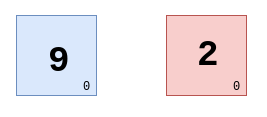
\includegraphics[scale=0.6]{JB_Prototype_Registers.png}
\end{figure}

Consider being shown these two colored boxes. The contents of the box are represented
as the large, centered numbers in bold. The indices of the box are represented as the
small number at the bottom right-hand corner. Indices tell you where to look in a
data structure (redundant for now, since registers only get one index).

\begin{itemize}
  \item Figure \ref{fig:Register_Indexing} shows how to access the 9 in the blue register.
  \begin{itemize}
    \item (called: blue sub 0)
  \end{itemize}
  \item Figure \ref{fig:Register_Indexing} also shows how to access the 2 in the red register.
  \begin{itemize}
    \item (called: red sub 0)
  \end{itemize}
\end{itemize}

\begin{figure}[!hb]
  \caption{Register Indexing}
  \label{fig:Register_Indexing}
  \centering
  
\includegraphics[scale=0.6]{JB_Prototype_Register_Indexing.png}
\end{figure}

From now on, these data structures of size 1, that only contains the index 0, will
be referred to as registers. A specific register and it's index is said to be a
memory location.\\

\textbf{Input}\\

Input is data that is given to you initially. This may include one regsiter or
multiple registers, as shown in Figure \ref{fig:Input_Example}.

\begin{figure}[!hb]
  \caption{Input Examples}
  \label{fig:Input_Example}
  \centering
  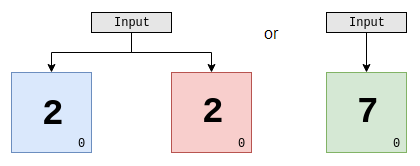
\includegraphics[scale=0.9]{JB_Prototype_Input.png}
\end{figure}

Input can also arrive in the form of an input stream. A stream of input is connected
to one register and continually pushes data from the stream into the register as
data is removed from it (see Figure \ref{fig:Input_Stream}). If there is no more data in the stream,
nothing will be pushed to the register.

\begin{figure}[!hb]
  \caption{Input Stream}
  \label{fig:Input_Stream}
  \centering
  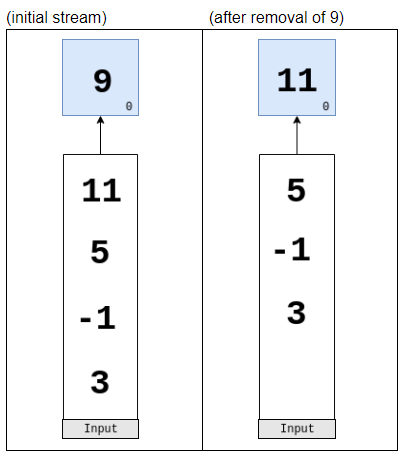
\includegraphics[scale=1]{JB_Prototype_Input_Stream.png}
\end{figure}
\vfill
\clearpage

\textbf{Output}\\

The output is checked at the end of the program. It is up to the player to link
the output to the correct data structure (only registers for now), as well as to
make sure the contents of the data structure match the expected output for the level.
A basic register to output linking can be seen in Figure \ref{fig:Output_Basic}.

\begin{figure}[!hb]
  \caption{Register to Output}
  \label{fig:Output_Basic}
  \centering
  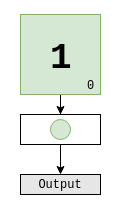
\includegraphics[scale=0.6]{JB_Prototype_Output_Basic.png}
\end{figure}

The green circle specifies that the contents of the green data structure will be
returned as the output for the player's solution to the puzzle level.\\

Consider a scenario in which multiple data structures may be returned as output.
In the following example (Figure \ref{fig:Output_Choice}), the player needs to return the register
with the greater value by choosing which colored data structure to link to the output.

\begin{figure}[!hb]
  \caption{Output Choice}
  \label{fig:Output_Choice}
  \centering
  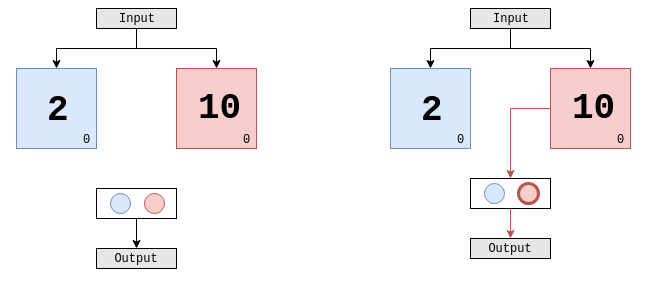
\includegraphics[scale=0.7]{JB_Prototype_Output_Choice.png}
\end{figure}

Players can link data structures to output by simply choosing the corresponding colored
circle of the data structure they would like to return. Clearly 10 is greater than 2 here and
the red register should returned.\\

\textbf{Instructions}\\

The notable instructions are as follows:

\begin{itemize}
  \item Move
  \item Return
  \item Add
  \item Subtract
  \item Jump
\end{itemize}

Instructions are clikced or dragged from a limited set of given instructions (
specific to each level).\\

When the player is ready to test their solution, each instruction will execute
procedurally from top to bottom.\\

It is up to us to structure the levels and instructions given in each level in such
a way that minimizes the amount of errors the player can create. Runtime errors
are okay, but we should strive to avoid having the player feel as if they are learning
syntax. We would also like to avoid confusing the player by giving a limited
instruction set for each level with thorough explanations for each instruction.\\

Paraneters used in certain instructions (Move, Return, Add, Subtract) are chosen
from a drop down menu, again minimizing the amount of errors the player can create
on their own. When choosing a colored data structure and an index, only the colors of
the data structures and their valid indices that are already on the puzzle board
are given as options in the drop down menu.\\
\newpage

\textbf{Instruction: Move}\\

The move instruction takes two arguments: a source register and a destination register.
It's main functionality consists of three different parts:

\begin{itemize}
  \item Moves the contents of the source to the destination.
  \item Leaves the contents of the source unchanged.
  \item Overrides whatever could have been in the destination previously.
\end{itemize}

How the instruction would look in the instruction editor is shown in Figure
\ref{fig:Move_Instruction}.

\begin{figure}[!hb]
  \caption{Move Instruction}
  \label{fig:Move_Instruction}
  \centering
  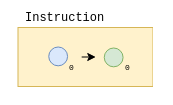
\includegraphics[scale=1]{JB_Prototype_Move.png}
\end{figure}

The contents of the two registers before and after the move instruction is
recieved is shown in Figure \ref{fig:Move_Instruction_Use}.

\begin{figure}[!hb]
  \caption{Move Instruction In Use}
  \label{fig:Move_Instruction_Use}
  \centering
  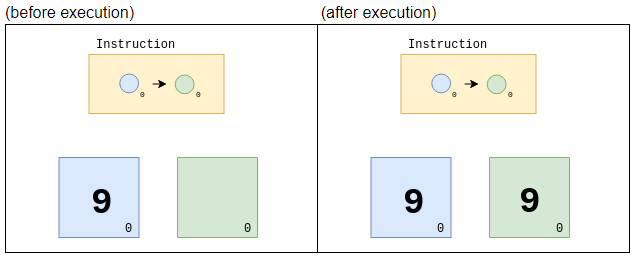
\includegraphics[scale=0.8]{JB_Prototype_Move_Use.png}
\end{figure}

Each argument (left and right side of the arrow) will have two drop down menus:
\begin{itemize}
  \item Color of register
  \item Index of register
\end{itemize}

The move instruction is atomic and meant to abstract the process of manually
picking up the data and placing it down.\\

\textbf{Instruction: Return}\\

The return instruction will specify only one arugment: which colored data structure
to return as output.
\begin{itemize}
  \item A return instruction is required for every level.
  \item May be given, or may ask the player to write it.
  \item The data structure that is returned is compared against the expected
  output for the level.
\end{itemize}

Figure \ref{fig:Return_Instruction} shows how the return instruction looks in the instruction editor.

\begin{figure}[!hb]
  \caption{Return Instruction}
  \label{fig:Return_Instruction}
  \centering
  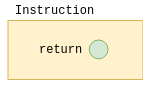
\includegraphics[scale=0.8]{JB_Prototype_Return.png}
\end{figure}

The argument is chosen from a drop down menu that allows the player to select
the color of the data structure they want to return.\\

Using the example from the output section (Figure \ref{fig:Output_Choice}),
we can show the correct usage of the return instruction in Figure \ref{fig:Return_Instruction_Use}.

\begin{figure}[!hb]
  \caption{Return Instruction In Use}
  \label{fig:Return_Instruction_Use}
  \centering
  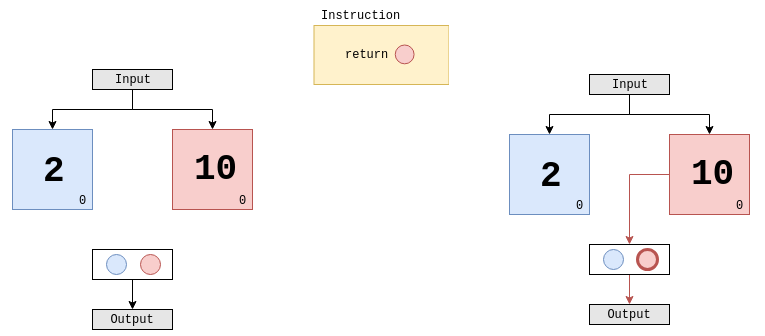
\includegraphics[scale=0.7]{JB_Prototype_Return_Use.png}
\end{figure}
\vfill
\clearpage

\textbf{Instruction: Add}\\

The add instruction takes three arguments:
\begin{itemize}
  \item Two memory locations to be added
  \item The destination of their sum (another memory location)
\end{itemize}

Figure \ref{fig:Add_Instruction} shows how the add instruction looks in the
instruction editor.

\begin{figure}[!hb]
  \caption{Add Instruction}
  \label{fig:Add_Instruction}
  \centering
  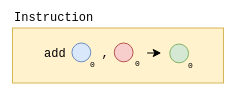
\includegraphics[scale=0.8]{JB_Prototype_Add.png}
\end{figure}

When referencing the memory locations, an index must also be specified (like we've
seen before). Figure \ref{fig:Add_Instruction_Use} shows the add instruction in use by displaying
the contents of the registers included in the instruction before and after it is
run.

\begin{figure}[!hb]
  \caption{Add Instruction In Use}
  \label{fig:Add_Instruction_Use}
  \centering
  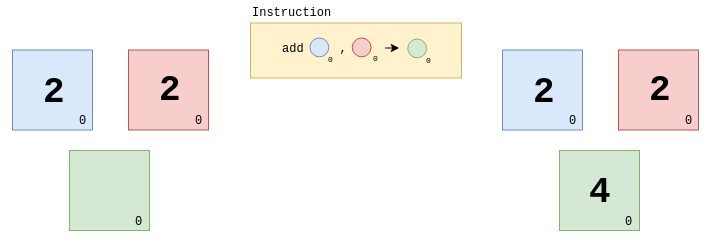
\includegraphics[scale=0.7]{JB_Prototype_Add_Use.png}
\end{figure}

Note:\\
The destination can be one of the source registers used, in which case it would
just overwrite the data similarly to how the move instruction does so.\\
\newpage

\textbf{Instruction: Subtract}\\

The subtract instruction works exactly the same as the add instruction above,
although the difference of the two reigsters is placed into the destination, rather
than the sum.\\

Figure \ref{fig:Sub_Instruction} shows how the subtract instruction looks in the
instruction editor.

\begin{figure}[!hb]
  \caption{Subtract Instruction}
  \label{fig:Sub_Instruction}
  \centering
  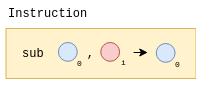
\includegraphics[scale=0.9]{JB_Prototype_Sub.png}
\end{figure}

\textbf{Instruction: Jump}\\

The jump instruction is paired with an anchor. When a jump instruction is executed,
the flow of control immediately jumps to the instruction that lays at the anchor.\\

It is up to the user to choose where the anchor will lie, after placing a Jump instruction
in the instruction editor.\\

Figure \ref{fig:Jump_Instruction} shows how the jump instruction looks in the
instruction editor.

\begin{figure}[!hb]
  \caption{Jump Instruction}
  \label{fig:Jump_Instruction}
  \centering
  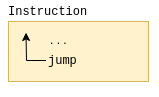
\includegraphics[scale=0.9]{JB_Prototype_Jump.png}
\end{figure}

Figure \ref{fig:Jump_Instruction_Use} shows how the control flow is handled when a jump instruction is
executed.

\begin{figure}[!hb]
  \caption{Jump Instruction In Use}
  \label{fig:Jump_Instruction_Use}
  \centering
  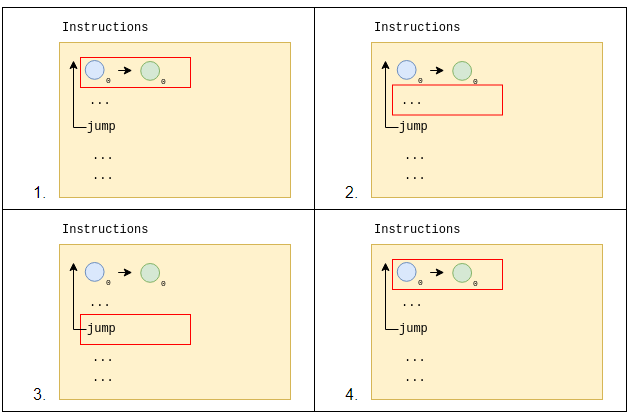
\includegraphics[scale=0.9]{JB_Prototype_Jump_Use.png}
\end{figure}
\vfill
\clearpage

\begin{figure}[!hb]
  \caption{Example Level: Find Sum}
  \label{fig:Find_Sum}
  \centering
  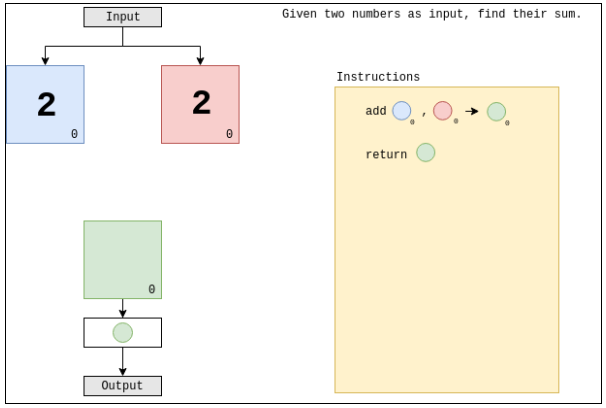
\includegraphics[scale=1]{JB_Prototype_Find_Sum.png}
\end{figure}
\vfill
\clearpage

\begin{figure}[!hb]
  \caption{Example Level: Return Last}
  \label{fig:Return_Last}
  \centering
  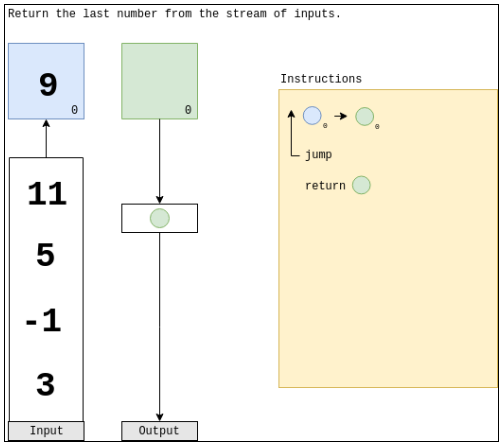
\includegraphics[scale=1]{JB_Prototype_Return_Last.png}
\end{figure}
\vfill
\clearpage

\newpage

\newpage

\subsubsection{Brandy King}
\todo{Create and format your LaTeX prototype write up here. Keep in mind that we
are currently in a subsubsection when labeling any headers (use paragraph and
subparagraph).}
\newpage

\newpage

\subsubsection{Nicolas LaCognata}
For my prototype, I spent a lot of time focusing on how we should integrate data structures into our assembly-based
puzzle structure. The approach I took saw players attaching data structures to registers to ``augment" them and
change how the register stores and processes information. I also took a stab at defining a theme for our game.\\

\textbf{Setting}\\
In \textit{Automata}, you play an Automaton stuck in a laboratory who is tasked with reprogramming itself to solve problems.
When solving the puzzle, they player may be addressed by a narrator when they make a mistake. The game was to have 
a ``Mad Science" feel to it, much like \textit{Portal}.\\

\textbf{Rules}\\
For each puzzle the player is presented with a problem, and they must use the provided instructions to solve it. 
Every puzzle will contain the following elements:
\begin{itemize}
	\item An Input track
	\item An Output track
	\item A set of static registers built into the test chamber
	\begin{itemize}
		\item These registers allow the player to store and manage multiple data cubes
	\end{itemize}
	\item A set of register augmenters
	\begin{itemize}
		\item These augmenters turn the registers into special data structures that can make the puzzles easier/possible
	\end{itemize}
	\item An instruction set
	\begin{itemize}
		\item These are the instructions the Automaton can execute to solve the puzzle; when placed in the solution window,
		they will be executed in the order they appear
		\item Some operations are invalid for certain states of the puzzle. For your safety, please avoid executing invalid operations.
	\end{itemize}
\end{itemize}
\newpage

\textbf{Instruction Set}
\begin{center}
    \begin{tabular}{ | m{3cm} | m{11cm} | } 
        \hline
            \begin{center}
                \textbf{INPUT} 
            \end{center}& 
            \textbf{Summary:} 
            \newline Allows your automata to grab an item from the input track. It places it in its hands.

            \textbf{Notes:} 
            \newline Your automata will drop any item currently in their hands to accept the new input, losing the old data forever.
            \newline If the input track is empty, the automata will do nothing

            \textbf{Faults:}
            \newline None\\
        \hline
            \begin{center}
                \textbf{OUTPUT} 
            \end{center}& 
            \textbf{Summary:} 
            \newline Allows your automata to place the item in its register into the output track.

            \textbf{Notes:} 
            \newline None

            \textbf{Faults:}
            \newline None\\
        \hline
            \begin{center}
                \textbf{SUBMIT} 
            \end{center}& 
            \textbf{Summary:} 
            \newline Allows your automata to submit its output for evaluation.

            \textbf{Notes:} 
            \newline This should always be the last instruction in your program.

            \textbf{Faults:}
            \newline Output Empty Error
            \newline Output Incorrect Error\\ 
        \hline
            \begin{center}
                \textbf{JUMP} 
            \end{center}& 
            \textbf{Summary:} 
            \newline This type of jump is unconditional. When your automata reads this instruction, it will move its instruction 
            counter to the corresponding anchor, effectively skipping forward or backward in your program.

            \textbf{Notes:} 
            \newline This instruction can be used to create loops.

            \textbf{Faults:}
            \newline Output Empty Error
            \newline Output Incorrect Error\\ 
        \hline
    \end{tabular}

    \begin{tabular}{ | m{3cm} | m{11cm} | } 
        \hline
            \begin{center}
                \textbf{JUMP IF NULL} 
            \end{center}& 
            \textbf{Summary:} 
            \newline This type of jump is conditional. When your automata reads this instruction, it will move its instruction counter 
            to the corresponding anchor, if and only if its hands are empty.

            \textbf{Notes:} 
            \newline This instruction can be used to exit loops when there is no more input.

            \textbf{Faults:}
            \newline None\\
        \hline
            \begin{center}
                \textbf{JUMP IF LESS X} 
            \end{center}& 
            \textbf{Summary:} 
            \newline This type of jump is conditional. When your automata reads this instruction, it will move its 
            instruction counter to the corresponding anchor, if and only if the data in its hand is less than the data in register X.

            \textbf{Notes:} 
            \newline This instruction can be used to exit loops or select branches of logic.

            \textbf{Faults:}
            \newline Hand Empty Error
            \newline Register Empty Error\\
        \hline
            \begin{center}
                \textbf{JUMP IF GREATER X} 
            \end{center}& 
            \textbf{Summary:} 
            \newline This type of jump is conditional. When your automata reads this instruction, it will move its instruction counter 
            to the corresponding anchor, if and only if the data in its hand is less than the data in register X.

            \textbf{Notes:} 
            \newline This instruction can be used to exit loops or select branches of logic.

            \textbf{Faults:}
            \newline Hand Empty Error
            \newline Register Empty Error\\
        \hline
    \end{tabular}

    \begin{tabular}{ | m{3cm} | m{11cm} | } 
        \hline
            \begin{center}
                \textbf{MOVETO X} 
            \end{center}& 
            \textbf{Summary:} 
            \newline This instruction allows your automata to place the item in its hand into a register on the board, specified by the argument X.

    
            \textbf{Notes:} 
            \newline This instruction overwrites any data in the target register, and empties your automata’s hand.
    
            \textbf{Faults:}
            \newline Hand Empty Error\\
        \hline
            \begin{center}
                \textbf{COPYTO X} 
            \end{center}& 
            \textbf{Summary:} 
            \newline This instruction allows your automata to copy the item in its hand into a register on the board, specified by the argument X.
    
            \textbf{Notes:} 
            \newline This instruction overwrites any data in the target register, but your automata retains a copy of the data.
    
            \textbf{Faults:}
            \newline Hand Empty Error\\
        \hline
            \begin{center}
                \textbf{MOVEFROM X} 
            \end{center}& 
            \textbf{Summary:} 
            \newline This instruction allows your automata to take an item from a register and keep it in its hand.

    
            \textbf{Notes:} 
            \newline This instruction overwrites any data the automata is holding and removes the data from the target register.
    
            \textbf{Faults:}
            \newline None\\
        \hline
            \begin{center}
                \textbf{COPYFROM X} 
            \end{center}& 
            \textbf{Summary:} 
            \newline This instruction allows your automata to copy an item from a register and keep it in its hand.
    
            \textbf{Notes:} 
            \newline This instruction overwrites any data the automata is holding, but the data also remains in the target register.
    
            \textbf{Faults:}
            \newline None\\
        \hline
    \end{tabular}

    \begin{tabular}{ | m{3cm} | m{11cm} | } 
        \hline
            \begin{center}
                \textbf{ADD X} 
            \end{center}& 
            \textbf{Summary:} 
            \newline This instruction allows your automata to add the value stored in a register to the value stored in its hand.
    
            \textbf{Notes:} 
            \newline The result of the operation is stored back in the automata’s hand.
    
            \textbf{Faults:}
            \newline Register Empty Error\\
        \hline
            \begin{center}
                \textbf{SUBTRACT X} 
            \end{center}& 
            \textbf{Summary:} 
            \newline This instruction allows your automata to subtract the value stored in a register to the value stored in its hand.

            \textbf{Notes:} 
            \newline The result of the operation is stored back in the automata’s hand.

            \textbf{Faults:}
            \newline Register Empty Error\\
        \hline
    \end{tabular}
\end{center}
\newpage
\newpage

\subsubsection{Sean Simonian}
\textbf{Paper Prototype 1.0}

My initial paper prototype, shown in Figure \ref{fig:Paper_Prototype_1.0}, built on the established game structure of manipulating input and output by executing instructions in a player's solution. The objective for each level is displayed at the top left of the screen, the solution space is on the right side, and the remaining area is utilized for visualizing the command execution. This prototype includes a robotic claw that can move horizontally across the top of the main game UI area, and can extend vertically to pick up or drop input values.

\begin{figure}[!hb]
  \caption{Paper Prototype 1.0}
  \label{fig:Paper_Prototype_1.0}
  \centering
  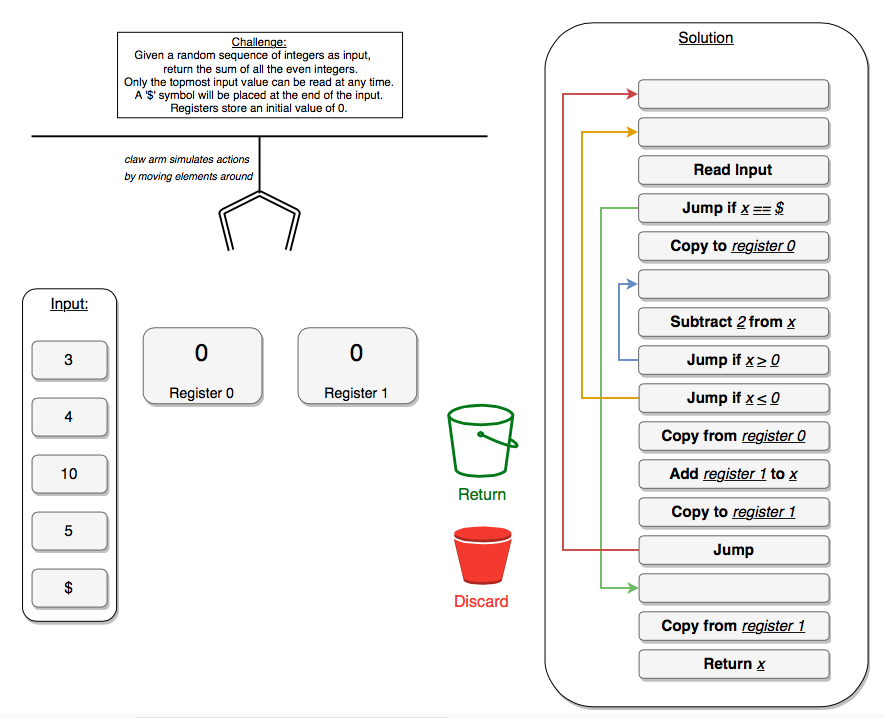
\includegraphics[scale=0.45]{SS_PP1.png}
\end{figure}


\paragraph{Solution Space:} ~\\
The solution space on the right side of the screen is where the player constructs their code-like solution to satisfy the puzzle objectives.
The player must use this space to place a series of instructions that will execute in order.

\paragraph{Instructions/commands:} ~\\
The instructions that are available in this prototype are:
\begin{itemize}
	\item Read Input
	\begin{itemize}
		\item The claw picks up the topmost item from the input.
	\end{itemize}
	\item Jump [If \_\_\_]
	\begin{itemize}
		\item This instruction will point to another line in the solution to jump to while executing.
		\item Optionally, the player may include an If \textit{condition}, so that the jump will only occur if a condition is met.
	\end{itemize}
	\item Copy \_\_\_ \_\_\_
	\begin{itemize}
		\item Copies the current value in the claw to a specified register, or copies the value from a register to the claw.
		\item The first blank can be set to either ``to'' or ``from''
		\item The second value can be set to a specific register
		\item Example: \textit{Copy to register 0}
	\end{itemize}
	\item Add \_\_\_
	\begin{itemize}
		\item Add the value of a specified register to the current value in the claw.
	\end{itemize}
	\item Subtract \_\_\_
	\begin{itemize}
		\item Subtract the value of a specified register from the current value in the claw.
	\end{itemize}
	\item Return
	\begin{itemize}
		\item Place the current value held by the claw into the return bin, and stop executing the instructions.
	\end{itemize}
\end{itemize}


\paragraph{The Claw:} ~\\
As each step of the player's solution is executed, the claw manipulates the data on the board, and the corresponding instructions are highlighted in the solution space.
The claw does all of the work manipulating data as it simulates the player's solution to the puzzle, and it can only hold at most one value at any time.
By having the claw hold a value and manipulate is as specified in the solution, this renders a separate ``current value'' box unnecessary.
The claw can pick up and put down data elements, or it can combine the element it's currently holding with another element to add or subtract values.

\paragraph{Input:} ~\\
Input arrives in a vertical stack that acts like a conveyor belt. The claw will navigate over the input stack, pick up the topmost item, and proceed to manipulate the data.

\paragraph{Registers:} ~\\
Registers are located in the middle of the game board, and they can be used to store data that needs to be set aside while the claw manipulates other data elements.

\paragraph{Discard Bin:} ~\\
Sometimes the current value being held by the claw is no longer needed, so it can be discarded in a trash can towards the bottom right of the screen. This gets rid of the value and can free up space for the claw or registers to hold useful elements.

\paragraph{Puzzle Description:} ~\\
Every puzzle has a clearly defined objective that should result in a single value to return upon completion, similar to a return value of a function in traditional programming. This prototype includes a ``return'' bin next to the discard bin, and the claw will place the final return value in the return bin to end the code execution. If the return value matches the expected value, then the solution was successful, otherwise the solution is incorrect.\\



\textbf{Paper Prototype 2.0: Puzzle Scene Design Concept}

After multiple iterations of prototype testing, team discussions to determine what works and what should be changed, we shared a solid view of how the puzzles should work, the components of included in the puzzles, the complete instruction set, etc.
This prototype, shown in Figure \ref{fig:Paper_Prototype_2.0}, was designed to present a possible view of what the entire level will look like, where the components are placed, how they interact with each other on screen, etc.


\begin{figure}[H]
  \caption{Paper Prototype 2.0}
  \label{fig:Paper_Prototype_2.0}
  \centering
  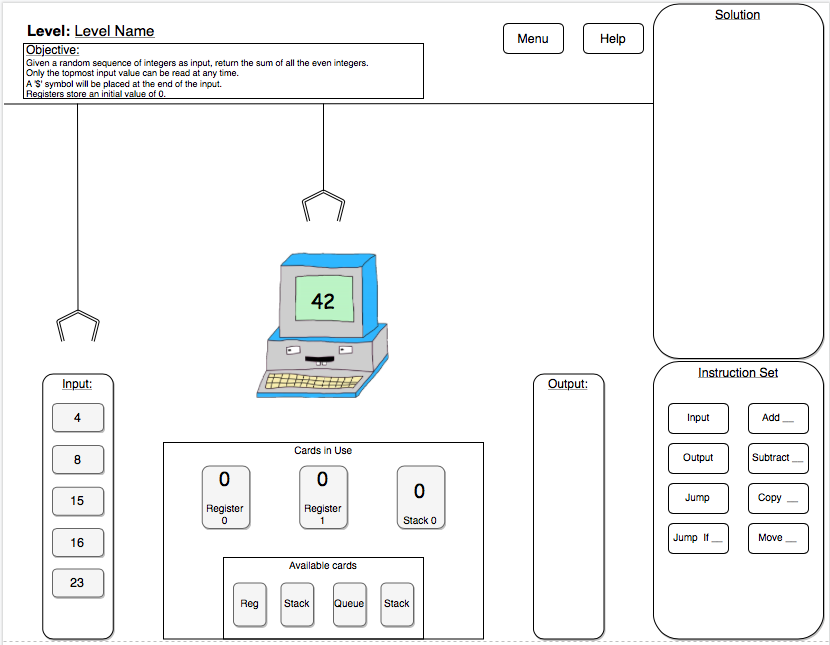
\includegraphics[scale=0.5]{SS_PP2.png}
\end{figure}


\paragraph{Menu Bar:} ~\\
The menu bar stretches across the top of the screen. This contains the name of the current level, along with some buttons to the right.
The Menu button will pause the game and bring up a pause menu, which will present the player with options to exit the puzzle, change game options, or resume the game.
The Help button can be pressed to give useful hints or tips for solving the puzzle if the player is struggling.


\paragraph{Level Description:} ~\\
Below the top menu bar is a section for the the description of the current level objectives. This will contain text that explains the current puzzle in a concise manner.


\paragraph{Solution Space:} ~\\
Similar to previous prototypes, the solution space on the right side is where the player constructs a solution to solve the puzzle objectives. This space includes a scrollbar on the right side to navigate long solutions.


\paragraph{Instruction Set:} ~\\
Below the solution space is the set of instructions the player can use for the current level.
The player can drag and drop these instructions into the solution space to construct their solution.
Dragging an instruction from the set creates a new instance of that instruction, meaning that the instruction does not get removed from the instruction set.
If the player clicks on an instruction, a description of that instruction will appear on the screen to remind the player what the instruction does and how to use it.


\paragraph{Game Space:} ~\\
The majority of the screen will be the game space, which contains the remaining elements which are explained below. The game space is where the remaining components interact to visually simulate the steps as the player's solution is executed.


\paragraph{The Claw:} ~\\
As each step of the player's solution is executed, the claw moves data between game components.
The claw moves horizontally along the top of the game space, and can expand/retract to reach components below it.
The claw is only used for transportation of data between two points, it does not hold onto anything when it is idle.
This means that any data that was picked up will be put down somewhere else before moving to the next step. Data is not modified while it is in the claw.


\paragraph{Computer:} ~\\
The central figure of this prototype design a sentient computer as a sort of actor.
The computer holds the current value that is displayed on its monitor, and it performs computations and manipulates data.
The claw can deliver data to the computer or pull data from the computer to move to another game component, such as a data structure or output.


\paragraph{Input:} ~\\
Input is received from a vertical stack or conveyor belt system on the bottom left of the game space.
The claw can pick up the topmost input value and move it somewhere else.


\paragraph{Output:} ~\\
Output is delivered to a vertical stack or conveyor belt system on the bottom right of the game space.
The claw can place a value onto the top of the output, and any prior output values slide downward or off the screen.


\paragraph{Card Space:} ~\\
The card space is at the bottom of the game space between input and output, and it displays the data structure cards that are available or in use.
The player can ``play'' a card by dragging and dropping an available card to the ``in use'' section.
Cards being used will display their contents, or if the data structure is too large to display, the player can click on the card to enlarge it and view the contents.
Players can also click on a card to get a description of the data structure and how to use it.



\newpage


\newpage

\subsection{Unified Prototype: Initial Game Structure}
\todo{Initial Game Structure...}
\newpage

\subsection{Game Mechanics}
\subsubsection{Tutorial Sequence}
\label{section:tutorial}
  The tutorial sequence of \textit{Computron} will introduce players to the game mechanics 
and allow players to acclimate to the puzzle solving workflow. The ordering of the tutorial 
sequence is crafted to control the rate at which players learn, and provide a smooth 
difficulty curve while constantly presenting new mechanics and concepts.\\

\paragraph{Level 1: Ins and Outs}
\subparagraph{Learning Objective:} Teach players the very basics of our user interface 
through a simple puzzle.

\subparagraph{Problem:} There is a single item in the input box. Please transfer it into 
the output box.

\subparagraph{Solution:} 
\begin{center}
    \begin{tabular}{ | m{5cm} | m{9cm} | } 
        \hline
            \textbf{Available Instructions:} 
            \begin{itemize}
                \setlength\itemsep{-.35em}
                \item INPUT
                \item OUTPUT
            \end{itemize}& 
            \textbf{Expected Solution:} 
            \begin{enumerate}
                \setlength\itemsep{-.35em}
                \item INPUT
                \item OUTPUT
            \end{enumerate}
            \\
        \hline
    \end{tabular}
\end{center}


\paragraph{Level 2: Ins and Outs pt. 2}
\subparagraph{Learning Objective:} Ensure that the player understands the basic 
mechanics of commanding Computron by requiring them to chain the previous 
puzzle's solution. In addition, prepare the player to understand the value of loops.

\subparagraph{Problem:} There are five items in the input box. Please transfer all 
of them into the output box.

\subparagraph{Solution:} 
\begin{center}
    \begin{tabular}{ | m{5cm} | m{9cm} | } 
        \hline
            \textbf{Available Instructions:} 
            \begin{itemize}
                \setlength\itemsep{-.35em}
                \item INPUT
                \item OUTPUT
            \end{itemize}& 
            \textbf{Expected Solution:} 
            \begin{enumerate}
                \setlength\itemsep{-.35em}
                \item INPUT
                \item OUTPUT
                \item INPUT
                \item OUTPUT
                \item INPUT
                \item OUTPUT
                \item INPUT
                \item OUTPUT
                \item INPUT
                \item OUTPUT
            \end{enumerate}
            \\
        \hline
    \end{tabular}
\end{center}

\paragraph{Level 2a (Optional): Alternator}
\subparagraph{Learning Objective:} Demonstrate a nuanced mechanic of the input 
instruction. It it not apparent from the previous puzzles, but executing two input 
commands in succession will cause Computron to discard the first.

\subparagraph{Problem:} There are 6 items in the input box. Please transfer every 
other item to the output box, starting with the second input.

\subparagraph{Solution:} 
\begin{center}
    \begin{tabular}{ | m{5cm} | m{9cm} | } 
        \hline
            \textbf{Available Instructions:} 
            \begin{itemize}
                \setlength\itemsep{-.35em}
                \item INPUT
                \item OUTPUT
            \end{itemize}& 
            \textbf{Expected Solution:} 
            \begin{enumerate}
                \setlength\itemsep{-.35em}
                \item INPUT
                \item INPUT
                \item OUTPUT
                \item INPUT
                \item INPUT
                \item OUTPUT
                \item INPUT
                \item INPUT
                \item OUTPUT
            \end{enumerate}
            \\
        \hline
    \end{tabular}
\end{center}
\newpage

\paragraph{Level 3: Hip Hop}
\subparagraph{Learning Objective:} Introduce the concept of jumping and looping.

\subparagraph{Problem:} There are 100 items in the input box. Please transfer each 
item to the output box, starting with the second input.

\subparagraph{Solution:} 
\begin{center}
    \begin{tabular}{ | m{5cm} | m{9cm} | } 
        \hline
            \textbf{Available Instructions:} 
            \begin{itemize}
                \setlength\itemsep{-.35em}
                \item INPUT
                \item OUTPUT
                \item JUMP
                \item JUMP IF NULL
            \end{itemize}& 
            \textbf{Expected Solution:} 
            \begin{enumerate}
                \setlength\itemsep{-.35em}
                \item INPUT
                \item JUMP IF NULL [EOP]
                \item OUTPUT
                \item JUMP 1
            \end{enumerate}
            \\
        \hline
    \end{tabular}
\end{center}

\paragraph{Level 4: Flip Flop}
\subparagraph{Learning Objective:} Introduce variable declaration, and present 
the player with their first significant challenge.

\subparagraph{Problem:} There are two items in the input box. Place them in the 
outbox in reverse order.

\newpage
\subparagraph{Solution:} 
\begin{center}
    \begin{tabular}{ | m{5cm} | m{9cm} | } 
        \hline
            \textbf{Available Instructions:} 
            \begin{itemize}
                \setlength\itemsep{-.35em}
                \item INPUT
                \item OUTPUT
                \item JUMP
                \item JUMP IF NULL
                \item MOVTO X
                \item MOVEFROM X
            \end{itemize}
            \textbf{Available Cards:} 
            \begin{itemize}
                \setlength\itemsep{-.35em}
                \item Register x2
            \end{itemize}& 
            \textbf{Expected Solution:} 
            \begin{enumerate}
                \setlength\itemsep{-.35em}
                \item Play Register [0]
                \item INPUT
                \item MOVETO [0]
                \item INPUT
                \item OUTPUT
                \item MOVEFROM [0] 
                \item OUTPUT
            \end{enumerate}
            \\
        \hline
    \end{tabular}
\end{center}

\paragraph{Level 5: Flip Flop Hop}
\subparagraph{Learning Objective:} Allow players to experiment with the new 
register mechanic, and guide them to generalize their previous solution.

\subparagraph{Problem:} There are 50 items in the input box. Place each pair of 
items in the inbox to the outbox in reverse order.

\subparagraph{Solution:} 
\begin{center}
    \begin{tabular}{ | m{5cm} | m{9cm} | } 
        \hline
            \textbf{Available Instructions:} 
            \begin{itemize}
                \setlength\itemsep{-.35em}
                \item INPUT
                \item OUTPUT
                \item JUMP
                \item JUMP IF NULL
                \item MOVTO X
                \item MOVEFROM X
            \end{itemize}
            \textbf{Available Cards:} 
            \begin{itemize}
                \setlength\itemsep{-.35em}
                \item Register x2
            \end{itemize}& 
            \textbf{Expected Solution:} 
            \begin{enumerate}
                \setlength\itemsep{-.35em}
                \item Play Register [0]
                \item INPUT
                \item JUMP IF NULL [EOP]
                \item MOVETO [0]
                \item INPUT
                \item OUTPUT
                \item MOVEFROM [0] 
                \item OUTPUT
                \item JUMP 2
            \end{enumerate}
            \\
        \hline
    \end{tabular}
\end{center}
\newpage

\paragraph{Level 6: Triceraflops}
\subparagraph{Learning Objective:} Expand player's understanding of the power 
of registers, and start guiding them toward seeing the value of stacks.

\subparagraph{Problem:} There are 3 items in the input box. Place all three in the 
output box in reverse order.

\subparagraph{Solution:} 
\begin{center}
    \begin{tabular}{ | m{5cm} | m{9cm} | } 
        \hline
            \textbf{Available Instructions:} 
            \begin{itemize}
                \setlength\itemsep{-.35em}
                \item INPUT
                \item OUTPUT
                \item JUMP
                \item JUMP IF NULL
                \item MOVTO X
                \item MOVEFROM X
            \end{itemize}
            \textbf{Available Cards:} 
            \begin{itemize}
                \setlength\itemsep{-.35em}
                \item Register x4
            \end{itemize}& 
            \textbf{Expected Solution:} 
            \begin{enumerate}
                \setlength\itemsep{-.35em}
                \item Play Register [0]
                \item Play Register [1]
                \item INPUT
                \item MOVETO [0]
                \item INPUT
                \item MOVETO [1]
                \item INPUT
                \item OUTPUT
                \item MOVEFROM [1] 
                \item OUTPUT
                \item MOVEFROM [0] 
                \item OUTPUT
            \end{enumerate}
            \\
        \hline
    \end{tabular}
\end{center}

\paragraph{Level 7: Triceraflops Hops}
\subparagraph{Learning Objective:} Force the player to generalize their previous 
solution for N inputs

\subparagraph{Problem:} There are 90 items in the input box. For each set of three 
in the inbox, transfer to the outbox in reverse order.

\newpage
\subparagraph{Solution:} 
\begin{center}
    \begin{tabular}{ | m{5cm} | m{9cm} | } 
        \hline
            \textbf{Available Instructions:} 
            \begin{itemize}
                \setlength\itemsep{-.35em}
                \item INPUT
                \item OUTPUT
                \item JUMP
                \item JUMP IF NULL
                \item MOVTO X
                \item MOVEFROM X
            \end{itemize}
            \textbf{Available Cards:} 
            \begin{itemize}
                \setlength\itemsep{-.35em}
                \item Register x4
            \end{itemize}& 
            \textbf{Expected Solution:} 
            \begin{enumerate}
                \setlength\itemsep{-.35em}
                \item Play Register [0]
                \item Play Register [1]
                \item INPUT
                \item JUMP IF NULL [EOP]
                \item MOVETO [0]
                \item INPUT
                \item MOVETO [1]
                \item INPUT
                \item OUTPUT
                \item MOVEFROM [1] 
                \item OUTPUT
                \item MOVEFROM [0]
                \item OUTPUT
                \item JUMP 3
            \end{enumerate}
            \\
        \hline
    \end{tabular}
\end{center}

\paragraph{Level 8: Fat Stacks}
\subparagraph{Learning Objective:} Introduce players to the Stack data structure, 
and demonstrate its FIFO property by having them reverse the input stream.

\subparagraph{Problem:} There are 6 items in the input box. Transfer each item into 
the outbox in reverse order.

\newpage
\subparagraph{Solution:} 
\begin{center}
    \begin{tabular}{ | m{5cm} | m{9cm} | } 
        \hline
            \textbf{Available Instructions:} 
            \begin{itemize}
                \setlength\itemsep{-.35em}
                \item INPUT
                \item OUTPUT
                \item JUMP
                \item JUMP IF NULL
                \item MOVTO X
                \item MOVEFROM X
            \end{itemize}
            \textbf{Available Cards:} 
            \begin{itemize}
                \setlength\itemsep{-.35em}
                \item Register x4
                \item Stack x1
            \end{itemize}& 
            \textbf{Expected Solution:} 
            \begin{enumerate}
                \setlength\itemsep{-.35em}
                \item Play Stack [0]
                \item INPUT
                \item JUMP IF NULL [6]
                \item MOVETO 0
                \item JUMP 2
                \item MOVEFROM [0]
                \item JUMP IF NULL [EOP]
                \item OUTPUT
                \item JUMP 6
            \end{enumerate}
            \\
        \hline
    \end{tabular}
\end{center}

\paragraph{Level 9: Comparatron}
\subparagraph{Learning Objective:} Introduce players to conditional jumps, and 
show that jumps can be used to select branches of logic.

\subparagraph{Problem:} The input box has two items in it. Output the greater of the two.

\newpage
\subparagraph{Solution:} 
\begin{center}
    \begin{tabular}{ | m{5cm} | m{9cm} | } 
        \hline
            \textbf{Available Instructions:} 
            \begin{itemize}
                \setlength\itemsep{-.35em}
                \item INPUT
                \item OUTPUT
                \item JUMP
                \item JUMP IF NULL
                \item JUMP IF LESS X
                \item JUMP IF GREATER X
                \item MOVTO X
                \item MOVEFROM X
            \end{itemize}
            \textbf{Available Cards:} 
            \begin{itemize}
                \setlength\itemsep{-.35em}
                \item Register x2
            \end{itemize}& 
            \textbf{Expected Solution:} 
            \begin{enumerate}
                \setlength\itemsep{-.35em}
                \item Play Register [0]
                \item INPUT
                \item MOVETO [0]
                \item INPUT
                \item JUMP IF GREATER [0], 7
                \item MOVEFROM [0]
                \item OUTPUT
            \end{enumerate}
            \\
        \hline
    \end{tabular}
\end{center}

\paragraph{Level 10: Big Fish}
\subparagraph{Learning Objective:} Allows players to generalize concept of maximization 
shown in the previous problem to a more robust situation, and continue making them 
comfortable with using jumps to select branches of logic.

\subparagraph{Problem:} The input box has some items in it. Output only the greatest 
number in the inbox.

\newpage
\subparagraph{Solution:} 
\begin{center}
    \begin{tabular}{ | m{5cm} | m{9cm} | } 
        \hline
            \textbf{Available Instructions:} 
            \begin{itemize}
                \setlength\itemsep{-.35em}
                \item INPUT
                \item OUTPUT
                \item JUMP
                \item JUMP IF NULL
                \item JUMP IF LESS X
                \item JUMP IF GREATER X
                \item MOVTO X
                \item MOVEFROM X
            \end{itemize}
            \textbf{Available Cards:} 
            \begin{itemize}
                \setlength\itemsep{-.35em}
                \item Register x2
            \end{itemize}& 
            \textbf{Expected Solution:} 
            \begin{enumerate}
                \setlength\itemsep{-.35em}
                \item Play Register [0]
                \item INPUT
                \item MOVETO [0]
                \item INPUT
                \item JUMP IF NULL 9
                \item JUMP IF LESS [0], 4
                \item MOVETO [0]
                \item JUMP 4
                \item MOVEFROM [0]
                \item OUTPUT
            \end{enumerate}
            \\
        \hline
    \end{tabular}
\end{center}

\paragraph{Level 10a (Optional): Two Fish}
\subparagraph{Learning Objective:} Allows players to challenge themselves with a 
more difficult variant of the previous problem.

\subparagraph{Problem:} The input box has some items in it. Output only the two 
largest numbers in ascending order.

\newpage
\subparagraph{Solution:} 
\begin{center}
    \begin{tabular}{ | m{5cm} | m{9cm} | } 
        \hline
            \textbf{Available Instructions:} 
            \begin{itemize}
                \setlength\itemsep{-.35em}
                \item INPUT
                \item OUTPUT
                \item JUMP
                \item JUMP IF NULL
                \item JUMP IF LESS X
                \item JUMP IF GREATER X
                \item MOVTO X
                \item MOVEFROM X
            \end{itemize}
            \textbf{Available Cards:} 
            \begin{itemize}
                \setlength\itemsep{-.35em}
                \item Register x4
            \end{itemize}& 
            \textbf{Expected Solution:} 
            \begin{enumerate}
                \setlength\itemsep{-.35em}
                \item Play Register [0]
                \item Play Register [1]
                \item Play Register [2]
                \item INPUT
                \item MOVETO [0]
                \item INPUT
                \item MOVETO [1]
                \item INPUT
                \item JUMP IF NULL 20
                \item JUMP IF LESS [0], 17
                \item MOVETO [2]
                \item MOVEFROM [0]
                \item MOVETO [1]
                \item MOVEFROM [2]
                \item MOVETO [0]
                \item JUMP 8
                \item JUMP IF LESS [1], 8
                \item MOVETO [1]
                \item JUMP 8
                \item MOVEFROM [1]
                \item OUTPUT
                \item MOVEFROM [0]
                \item OUTPUT
            \end{enumerate}
            \\
        \hline
    \end{tabular}
\end{center}

\paragraph{Level 10b (Optional): Red Fish}
\subparagraph{Learning Objective:} Allows players to challenge themselves with a 
more difficult variant of the previous two problems. Lead them to see the value of 
max heaps.

\subparagraph{Problem:} The input box has some items in it. Output only the three 
largest numbers in ascending order.

\newpage
\subparagraph{Solution:} 
\begin{center}
    \begin{tabular}{ | m{5cm} | m{9cm} | } 
        \hline
            \textbf{Available Instructions:} 
            \begin{itemize}
                \setlength\itemsep{-.35em}
                \item INPUT
                \item OUTPUT
                \item JUMP
                \item JUMP IF NULL
                \item JUMP IF LESS X
                \item JUMP IF GREATER X
                \item MOVTO X
                \item MOVEFROM X
            \end{itemize}
            \textbf{Available Cards:} 
            \begin{itemize}
                \setlength\itemsep{-.35em}
                \item Register x4
            \end{itemize}& 
            \textbf{Expected Solution:} 
            \begin{enumerate}
                \setlength\itemsep{-.60em}
                \item Play Register [0]
                \item Play Register [1]
                \item Play Register [2]
                \item Play Register [3]
                \item INPUT
                \item MOVETO [0]
                \item INPUT
                \item MOVETO [1]
                \item INPUT
                \item MOVETO [2]
                \item INPUT
                \item JUMP IF NULL 32
                \item JUMP IF LESS [0], 22
                \item MOVETO [3]
                \item MOVEFROM [1]
                \item MOVETO [2]
                \item MOVEFROM [0]
                \item MOVETO [1]
                \item MOVEFROM [3]
                \item MOVETO [0]
                \item JUMP 11
                \item JUMP IF LESS [1], 28
                \item MOVETO [3]
                \item MOVEFROM [1]
                \item MOVETO [2]
                \item MOVEFROM [3]
                \item MOVETO [1]
                \item JUMP 11
                \item JUMP IF LESS [2], 11
                \item MOVETO 2
                \item JUMP 11
                \item MOVEFROM [2]
                \item OUTPUT
                \item MOVEFROM [1]
                \item OUTPUT
                \item MOVEFROM [0]
                \item OUTPUT
            \end{enumerate}
            \\
        \hline
    \end{tabular}
\end{center}

\paragraph{Level 11: You Fish}
\subparagraph{Learning Objective:} Introduce players to their second data structure, the heap.

\subparagraph{Problem:} Place all the items in the inbox into the outbox in descending order.

\newpage
\subparagraph{Solution:} 
\begin{center}
    \begin{tabular}{ | m{5cm} | m{9cm} | } 
        \hline
            \textbf{Available Instructions:} 
            \begin{itemize}
                \setlength\itemsep{-.35em}
                \item INPUT
                \item OUTPUT
                \item JUMP
                \item JUMP IF NULL
                \item JUMP IF LESS X
                \item JUMP IF GREATER X
                \item MOVTO X
                \item MOVEFROM X
            \end{itemize}
            \textbf{Available Cards:} 
            \begin{itemize}
                \setlength\itemsep{-.35em}
                \item Register x4
                \item Max Heap x1
            \end{itemize}& 
            \textbf{Expected Solution:} 
            \begin{enumerate}
                \setlength\itemsep{-.35em}
                \item Play Max Heap [0]
                \item INPUT
                \item JUMP IF NULL 6
                \item MOVETO [0]
                \item JUMP 2
                \item MOVEFROM [0]
                \item JUMP IF NULL [EOP]
                \item OUTPUT
            \end{enumerate}
            \\
        \hline
    \end{tabular}
\end{center}

\paragraph{Level 12: Sad Fish}
\subparagraph{Learning Objective:} Show players the power of combining data 
structures to accomplish a new task.

\subparagraph{Problem:} Place all the items in the inbox into the outbox in ascending order.

\newpage
\subparagraph{Solution:} 
\begin{center}
    \begin{tabular}{ | m{5cm} | m{9cm} | } 
        \hline
            \textbf{Available Instructions:} 
            \begin{itemize}
                \setlength\itemsep{-.35em}
                \item INPUT
                \item OUTPUT
                \item JUMP
                \item JUMP IF NULL
                \item JUMP IF LESS X
                \item JUMP IF GREATER X
                \item MOVTO X
                \item MOVEFROM X
            \end{itemize}
            \textbf{Available Cards:} 
            \begin{itemize}
                \setlength\itemsep{-.35em}
                \item Register x4
                \item Max Heap x1
                \item Stack x1
            \end{itemize}& 
            \textbf{Expected Solution:} 
            \begin{enumerate}
                \setlength\itemsep{-.35em}
                \item Play Max Heap [0]
                \item Play Stack [1]
                \item INPUT
                \item JUMP IF NULL 7
                \item MOVETO [0]
                \item JUMP 3
                \item MOVEFROM [0]
                \item JUMP IF NULL [11]
                \item MOVETO [1]
                \item JUMP [7]
                \item MOVEFROM [1]
                \item JUMP IF NULL [EOP]
                \item OUTPUT
                \item JUMP 11
            \end{enumerate}
            \\
        \hline
    \end{tabular}
\end{center}
\newpage

\newpage

\section{System Design}
  \subsection{Developer Tools}
When brainstorming the requirements for \textit{Computron}, a great deal of thought was put into the selection of developer tools. As the team has learned, choosing the wrong tool can be a very expensive mistake. Two of the most vital choices we made, the engine and the version control system, are documented in this section.

\subsubsection{Game Engine} \label{game_engine}
Making games from scratch is a long and difficult practice. Like most small development teams, we decided from day one that making a custom framework or engine would be inappropriate for the scope of the project. The team decided instead to make use of a commercial game engine. Using a commercial game engine puts a huge set of tools at our disposal, and allows for rapid prototyping and iterations. However, choosing which game engine to use is still a non-trivial solution. When choosing to use a commercial game engine, there are two major options: Unreal Engine 4 (developed by Epic Games) and Unity (developed by Unity Technologies). Both engines are excellent choices, and we carefully weighed their positive and negative attributes. 

Unreal Engine 4 is a high power tool. Written and scripted in C++, games shipped with Unreal can push the limits of the player's computer hardware. In addition Unreal is open source, includes better support for version control, and provides a very mature visual scripting system to aid in producing game logic. However, concerns were raised that Unreal would be too powerful for the needs of our project. Unreal's higher graphical fidelity is irrelevant in a sprite-based 2D application, and the engine's generally steeper learning curve threatened to greatly slow our progress in the project's early stages. In addition, Unreal's huge C++ code base can often result in very long compile times, especially for older development machines.

Unity is also an extremely advanced tool. Written in C++ and scripted with C\#, games made with Unity can generally be prototyped and iterated much faster than Unreal Projects. Unity easier to learn, has better documentation, more tutorials, and has vastly superior support for 2D titles. However, Unity's poor support for modern, non-proprietary version control systems borders inexcusable. The lack of a visual scripting tool can also prove cumbersome for some gameplay programming tasks that deal in more abstract ideas like game flow and artificial intelligence.

After extensive discussions, it was unanimously decided that \textit{Computron} will be built using Unity, version 2019.2.12.f1. Improved support for 2D titles and and superior ease of use were the deciding factors.





\subsubsection{Version Control System}
Choosing Unity as our game's engine made choosing the right version control system for \textit{Computron} an extremely difficult process. The Unity Editor's heavy use of binary files, and its tendency to generate lots of temporary files between program runs made integrating traditional version control systems like Git and Subversion difficult. Unity's solution to it's difficult relationship with version control systems is Unity Collaborate, however a quick evaluation of its features proved it to be an insufficient solution to the teams requirements. Unity Collaborate lacks many basic features of any modern version control system, including: 

\begin{enumerate}
    \item Branching and Merging.
    \item Any out of Editor interface to the repository.
    \item Single file reverts/restores.
    \item Support for more than 3 team members without paying money.
    \item Access to more than 1GB of server space without playing money.
    \item Ability to host a dedicated server.
\end{enumerate}

Despite the troubles presented, we still decided  to use Git. Using Git for version control worked extremely well during the first sprint, up until our first major integration, it then became clear that Git support was worse than expected. Even after configuring the editor to use plain-text meta files and assets, Git was entirely unable to merge non-conflicting changes in a single Unity scene. Workarounds existed to make Git compatible with these scene merge conflicts, but the process did not work consistently on both Mac and Windows dev machines.

In place of hacking together a a git integration, the team decided to migrate to Perforce. Unity has minor built in support for Perforce, and recently released that support for the free tier of the editor. Perforce is the dominant version control system in the games industry, and is free for small student teams. Unlike Git, perforce does not have a standard (and free) cloud platform for hosting repositories. Perforce administrators are expected to find their own server space. \textit{Computron's} perforce repository is hosted on a free Amazon Web Service EC2 Linux server. The AWS server has proved highly accessible, configurable, and performant. 

Our Perforce configuration has proven stable on both Windows and Mac development machines, and has allowed us to collaborate without any major incidents. Perforce has an extensive feature set for working with the binary files often found in game repositories, and allows users to lock files and force sequential edits when making breaking changes.


\newpage

\subsection{Overall Project Structure}
At the highest level, our game is organized into several major systems that communicate between three Unity Scenes: the Save-Load system, the Level Generation System, the Puzzle System, the Puzzle User Interface, the Interpreter, and the Actor. A graphical representation of the relationship between these systems is show in figure \ref{fig:overall_system_diagram}.

\begin{figure}[!hb]
    \caption{Computron System Overview}
    \label{fig:overall_system_diagram}
    \centering
    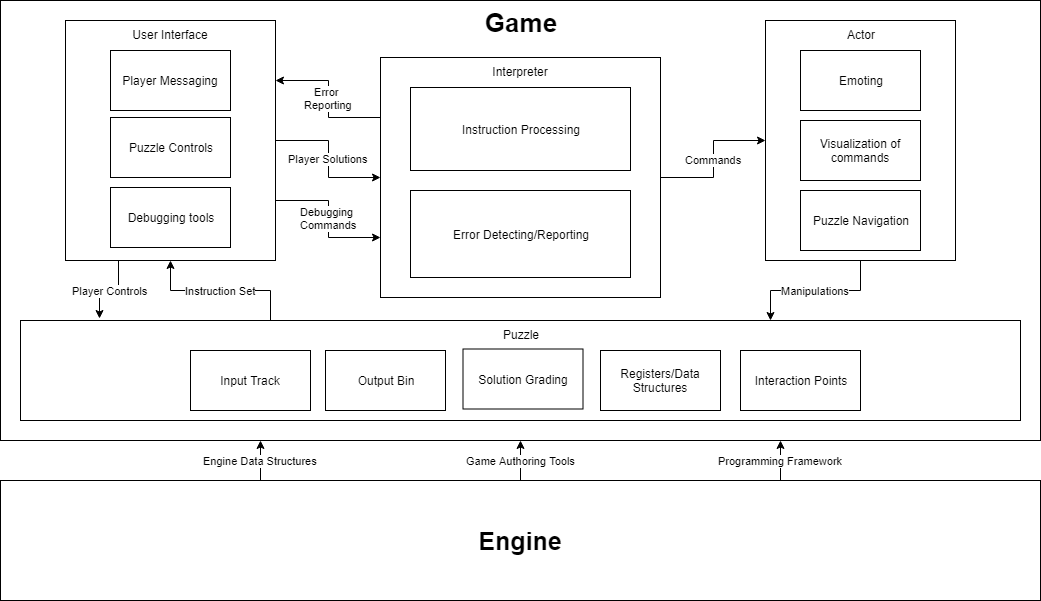
\includegraphics[width=\textwidth]{Diagrams/SystemDiagram.png}
\end{figure}

A more detailed explanation of all of these systems can be found throughout the remainder of this section.
\newpage

\subsection{Save Load System}
\subsubsection{Overview}
The Save-Load system is the backbone of Computron. It is responsible for serializing and deserializing all the relevant player data needed to reconstruct play sessions. The system currently supports up to three player save slots to store game data. This restriction is an artificial one, as we only chose to allow the UI of the main menu to address three slots. The underlying mechanisms of the system can handle arbitrarily many save slots, as long as the player is given an interface to select them. An overview is provided by \ref{fig:saveload_system_diagram}.

\begin{figure}[!hb]
    \caption{Save-Load System Overview}
    \label{fig:saveload_system_diagram}
    \centering
    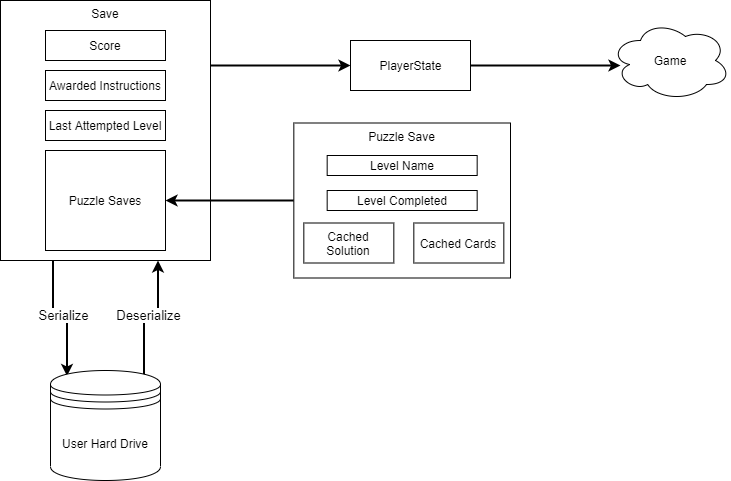
\includegraphics[width=\textwidth]{Diagrams/SaveLoad.png}
\end{figure}

As hinted to above, the only place in which the player actively interacts with the Save-Load system is at game startup. After hitting play, the player will be presented with a choice of three save slots, and the necessary UI to create, delete, or select a save in any of the three slots. 

\subsubsection{Data}
In this section you will find an enumeration of all the information required to restore user play sessions. Due to how this information is generated and captured, changes to the game's level layout can corrupt these save files and cause unexpected behavior in the level selection scene and puzzle scenes. It is highly recommended that developers clear outdated save files when adding, removing, or otherwise altering levels.

The top-level save object is simply called a Save. Below is an enumeration of the data captured in a save:
\begin{itemize}
    \item Player Score
    \item Awarded Instructions
    \item Last Attempted Level
    \item A collection of puzzle-specific saves for each puzzle the player has attempted
\end{itemize}

Top-level Saves defer the responsibility of tracking per-puzzle player data to a specialized serializable object cleverly know as a Puzzle Save. Puzzle Saves are generated and maintained on a per-level basis. When a player visits a level for the first time, a new entry is added to their save file for that level. This entry includes the following information:
\begin{itemize}
    \item The level's name
    \item Whether the level has been completed
    \item A list of what instructions the player left in the solution window
    \item A list of what cards the player left in the play area
    \item Which challenge stars the player has earned
\end{itemize}

\subsubsection{Scene Traversal}
After all this data is collected, and loaded (from either a binary or JSON save file) it is transferred to a PlayerState GameObject which travels between all scenes. This PlayerState object provides an interface for level generation systems read and write from player session data to configure the scenes and report significant game events.
\newpage

\subsection{Level Generation System}
\subsubsection{Overview}
Player save information is not the only information to traverse scenes. In order to allow 25 different puzzles to be displayed on the same Unity scene, \textit{Computron} makes heavy use of an enumeration of puzzle data, and a Puzzle Generator that processes that data to configure the puzzle scene for the selected puzzle.

This information is embedded in the all of the GameObjects used to create the level select graph. These nodes of the graph serve two purposes. The root GameObject of each node contains all of the data required to maintain the level graph. This includes an adjacency list of neighbors, components required to render and draw lines between the nodes, and an integer value specifying the required score to make that node traversable. Attached as a payload to each of these nodes is a child GameObject that contains the enumeration of all the data required to generate   

\subsubsection{Data}
The enumeration of all the data required to generate a level can be found via the public members of the Puzzle Data. This data includes:

\begin{itemize}
    \item Puzzle name
    \item Puzzle prompt
    \item The type of Output Generator to use
    \item Puzzle hints
    \item Number of each card type allowed in the puzzle
    \item Which challenge stars are available for the level
    \item The score threshold for each enabled challenge star
    \item A flag to generate random input
    \item A seed for the input random number generator
    \item A seed for the card address random number generator
    \item The number of inputs to generate for this puzzle
    \item (Optional) an explicit input sequence to use in place of random numbers
    \item Instruction filtering flags to enable or disable parts of the CAL 
    \item A Tutorialization script to specify an interactive tutorial sequence
\end{itemize}

Manipulating the data structure above, and correctly connecting a prefabricated map node to the level graph are the only two steps required to add a basic puzzle to the game.

\subsubsection{Scene Traversal}
In order to feed puzzle information to the puzzle scene, that data object of a selected level node is extracted from the instance of the level graph and persisted to the Puzzle Scene for puzzle generation.
\newpage

\subsection{Puzzle System}
\subsubsection{Overview}
Our puzzle system will be responsible for formally defining the nature and
functionality of the puzzles in our game.\\

The following diagram, Figure \ref{fig:puzzle_system_diagram}, gives a general overview of the components
of the puzzle system and how they communicate with one another.

\begin{figure}[!hb]
  \caption{Puzzle System Overview}
  \label{fig:puzzle_system_diagram}
  \centering
  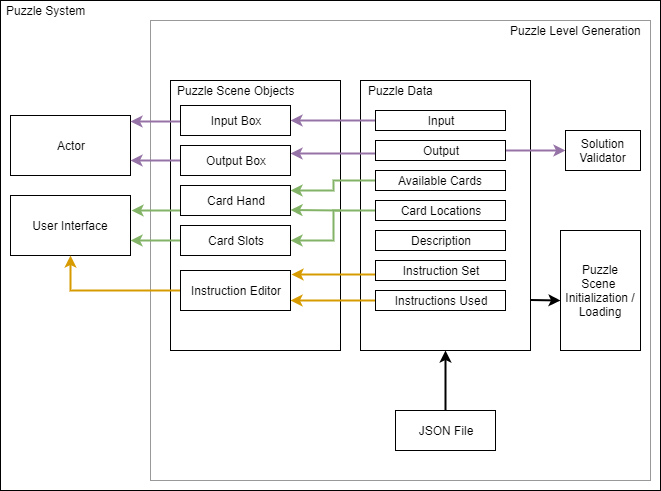
\includegraphics[scale=0.6]{Diagrams/puzzle_system_diagram.png}
\end{figure}
\vfill
\clearpage

The responsibilities of the puzzle system are as follows:

\begin{itemize}
	\item Present input to the player
	\item Determine the expected output the player is responsible for generating
		% what does the following line mean?
	\item Decide the question we can ask the player
	\item Offer allowed operations the player can perfrom to solve the puzzle
	\item Load an initial puzzle scene specific to each puzzle level
	\item Save a puzzle scene state for a specific level when the player leaves
	\item Load saved puzzle scene states for each level a player has previously attempted
\end{itemize}

Here are the main components of the Puzzle Scene that rely on the Puzzle System:

\begin{itemize}
	\item Input / Output (I/O)
	\begin{itemize}
		\item Input Box
		\item Output Box
		\item I/O Data (numbers)
	\end{itemize}

	\item Game Cards
	\begin{itemize}
		\item Player Card Hand
		\item Card Slots
	\end{itemize}

	\item Instruction Area
	\begin{itemize}
		\item Instruction bank
	\end{itemize}
\end{itemize}

Note:\\

While the Game Cards and the Instruction Area fall under the User
Interface System, there are certain parts of these components that rely on
the Puzzle System’s level generation functionalities. Only that relationship
will be mentioned here. Refer to the User Interface System for a more detailed
look at these game components.

\subsubsection{Puzzle Level Generation}
When a level is chosen to be played by the player, the puzzle system controls
which game objects get loaded on to the puzzle Scene. This process is handled
by a puzzle generation script that reads JSON data associated to the specific
level that was chosen.

\subsubsection{Level Initialization/Loading}
The generator will either load or initialize a puzzle level depending on whether
or not the player has previously attempted to solve the puzzle level. This
decision process is exemplified in Figure \ref{fig:json_decision_diagram}.\\

If the JSON file does not exist, the player has never attempted the chosen level before. The
generator will then need to call upon a level initialization script that will
create a JSON file for the level that represents its initial state. After the file
is written, its data is loaded by the generator and the puzzle Scene is loaded.
This sequence is shown in Figure \ref{fig:level_initialization_diagram}.\\

If the JSON file does exist, the generator simply skips the initialize step and
loads the puzzle Scene state based on the file that was found for the level (as
shown in Figure \ref{fig:level_loading_diagram}).\\

This flow of control combines initialization and loading processes in order to simplify
the entire scheme. The only difference between the two is the possible need to
initially create a level's JSON file, but that created file, or the one that already
existed under the same name, is always loaded by the generator.\\

When a game is ran for the first time, there will be no JSON files associated to
ANY level. This means that the level initialization script will be invoked each time
the player opens a new level, as expected.\\

\begin{figure}[!hb]
  \caption{Puzzle Level Initialization/Loading Decision}
  \label{fig:json_decision_diagram}
  \centering
  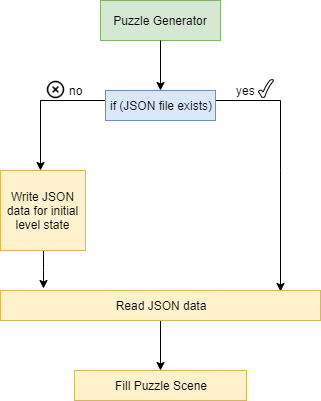
\includegraphics[scale=0.9]{Diagrams/json_decision_diagram.png}
\end{figure}
\vfill
\clearpage

\begin{figure}[!hb]
  \caption{Puzzle Level Initialization}
  \label{fig:level_initialization_diagram}
  \centering
  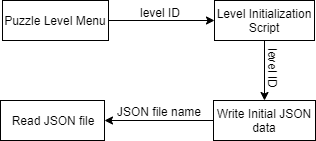
\includegraphics[scale=0.9]{Diagrams/level_initialization_diagram.png}
\end{figure}

\begin{figure}[!hb]
  \caption{Puzzle Level Loading}
  \label{fig:level_loading_diagram}
  \centering
  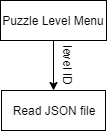
\includegraphics[scale=0.9]{Diagrams/level_loading_diagram.png}
\end{figure}
\vfill
\clearpage

\subsubsection{Level Saving}
When the player decides to leave a puzzle level (via exiting the game, returning to the
level menu, etc), the puzzle system saves the state of the current level by writing
to the JSON file associated to it. Figure \ref{fig:level_saving_diagram} shows this process.

\begin{figure}[!hb]
  \caption{Puzzle Level Saving}
  \label{fig:level_saving_diagram}
  \centering
  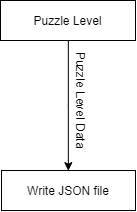
\includegraphics[scale=0.9]{Diagrams/level_saving_diagram.png}
\end{figure}

\subsubsection{JSON File Format}
The JSON file is serialized using a PuzzleData object that contains information
needed to fill the puzzle scene. This data can be separated into two categories:\\

Data Needed for Level State Initialization:
\begin{itemize}
  \item Initial cards in hand
  \item Number of register cards available
  \item Number of stack cards available
  \item Number of queue cards available
  \item Number of heap cards available
  \item Input size
  \item Instruction set
  \item Puzzle description
\end{itemize}

Data Needed for Loading a Previous Level State:
\begin{itemize}
  \item Card placement
  \item Cards in hand
  \item Instructions in editor
\end{itemize}

\subsubsection{Input}
The Puzzle System is in charge of filling the puzzle Scene's input box with data
that is necessary for the chosen level. As shown by Figure \ref{fig:Puzzle_System_Input_Overview}, 
the puzzle generator takes an input size \textit{n} from the JSON file and randomly generates an array of 
\textit{n} numbers that is used to fill the input box with corresponding data. A more visualized
look at how the input box game object is filled is shown in Figure \ref{fig:Puzzle_System_Input_Same_Before}.\\

\begin{figure}[!hb]
  \caption{Puzzle System: Input Overview}
  \label{fig:Puzzle_System_Input_Overview}
  \centering
  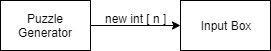
\includegraphics[scale=0.9]{Diagrams/Puzzle_System_Input_Overview.png}
\end{figure}

The puzzle system is responsible for giving the actor the correct data from the
input box when it is needed. The actor can make an input request to the input box.
The system will simply return the top-most element from the input box to the actor entity, along with the
numerical data that is associated with it behind the scenes (see Figure \ref{fig:Puzzle_System_Input_Actor}).\\

Note:\\

If the Actor makes an input request to an empty input box, the puzzle system
will return NULL.\\

The input box has a fixed number of input items that can fit inside (5 in our examples).
Sometimes the size of the input stream can be larger than the size of the input box
itself. In this case, the input box works as a queue. If we had an input stream of
size 6, the 6th element would be hidden until the top-most element of the input box
is removed by the actor. All of the elements below will move up a slot and the
hidden 6th element would then appear at the bottom, as shown in Figure \ref{fig:Puzzle_System_Input_Overload_Before} and
Figure \ref{fig:Puzzle_System_Input_Overload_After}.\\

If the input stream is the same size as the input box, or if the actor has removed
enough numbers from a larger stream and there are no more slots to fill, the input numbers
behave only slightly differently. Figure \ref{fig:Puzzle_System_Input_Same_Before}
and Figure \ref{fig:Puzzle_System_Input_Same_After} show how the numbers below will move up a slot, like before,
but the bottom slot will be left empty.\\

\begin{figure}[!hb]
  \caption{Input-Box/Actor Communication}
  \label{fig:Puzzle_System_Input_Actor}
  \centering
  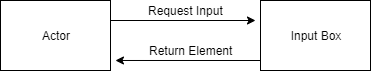
\includegraphics[scale=0.9]{Diagrams/Puzzle_System_Input_Actor.png}
\end{figure}

\begin{figure}[!hb]
  \caption{Input-Box Overloading (before)}
  \label{fig:Puzzle_System_Input_Overload_Before}
  \centering
  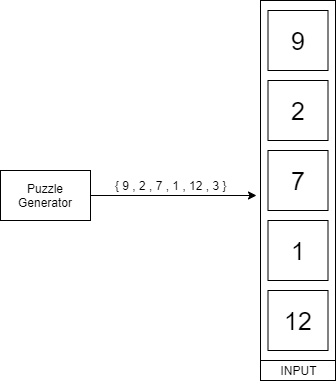
\includegraphics[scale=0.9]{Diagrams/Puzzle_System_Input_Overload_Before.png}
\end{figure}

\begin{figure}[!hb]
  \caption{Input-Box Overloading (after)}
  \label{fig:Puzzle_System_Input_Overload_After}
  \centering
  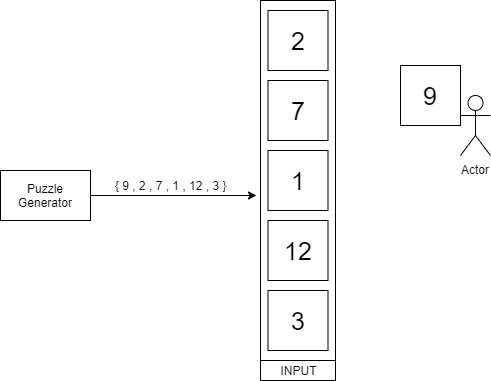
\includegraphics[scale=0.9]{Diagrams/Puzzle_System_Input_Overload_After.png}
\end{figure}
\vfill
\clearpage

\begin{figure}[!hb]
  \caption{Input-Box Same Size (before)}
  \label{fig:Puzzle_System_Input_Same_Before}
  \centering
  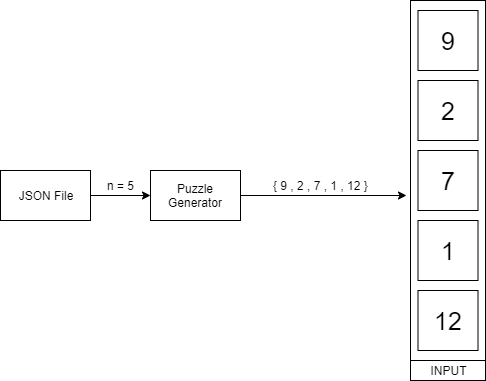
\includegraphics[scale=0.9]{Diagrams/Puzzle_System_Input_Same_Before.png}
\end{figure}

\begin{figure}[!hb]
  \caption{Input-Box Same Size (after)}
  \label{fig:Puzzle_System_Input_Same_After}
  \centering
  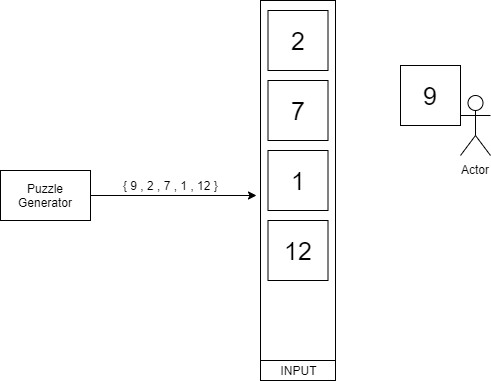
\includegraphics[scale=0.9]{Diagrams/Puzzle_System_Input_Same_After.png}
\end{figure}
\vfill
\clearpage

\subsubsection{Output}
In regards to output, the Puzzle System handles the interaction points between:
\begin{itemize}
  \item The output box
  \item The Actor
  \item The output validator
\end{itemize}
The Actor, after recieving an output instruction from the Interpreter, places the
data item from its hands to the output box. After all of the instructions are run, the
entire contents of the output box are submitted for validation, as shown in Figure
\ref{fig:Puzzle_System_Output_Interaction}.\\

The puzzle generation script generates the expected output based on the input that
was also generated previously. An output validation script takes the contents of
the player's output box, their solution, and compares it against the expected output.
If the contents match, the player has solved the puzzle. If the contents do not match,
the player's solution did not solve the puzzle. Figure \ref{fig:Puzzle_System_Output_Validation} shows this decision process.

\begin{figure}[!hb]
  \caption{Output Interaction Points}
  \label{fig:Puzzle_System_Output_Interaction}
  \centering
  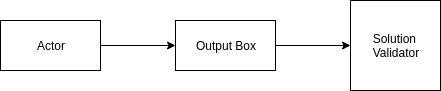
\includegraphics[scale=0.9]{Diagrams/Puzzle_System_Output_Interaction.png}
\end{figure}

\begin{figure}[!hb]
  \caption{Output Validation}
  \label{fig:Puzzle_System_Output_Validation}
  \centering
  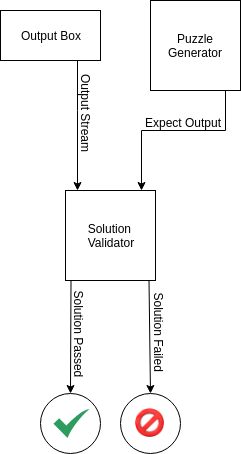
\includegraphics[scale=0.9]{Diagrams/Puzzle_System_Output_Validation.png}
\end{figure}
\vfill
\clearpage

\subsubsection{Game Cards}
The Puzzle System makes use of the puzzle generator in order to tell the user interface
which game cards are placed in certain positions on the game board when beginning
or loading a level. Card positions are pulled from the current level's JSON file.
A card position not only indicates if a card is in the player's card hand or the puzzle board's
card slots, but also the position within either of those areas.\\

The card hand is filled during initialization. The JSON file will contain the following:
\begin{itemize}
   \item Number of register cards
   \item Number of stack cards
   \item Number of queue cards
   \item Number of heap cards
\end{itemize}

The intitial content of the card hand is based on this data, although the locations
of these cards may be changed later on.\\

Any update to a card's position will be reflected when returning to that level.
When a level is exited, all of the cards locations on the game board are saved to
that level's JSON file. When a level is loaded at another point in time, the card
objects will be instantiated based on their locations, rather than the number of
each card like above.\\

\begin{figure}[!hb]
  \caption{Game Card Position Loading/Intializing}
  \label{fig:Puzzle_System_Cards}
  \centering
  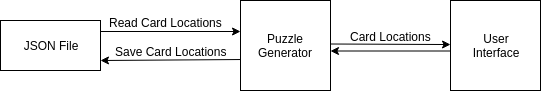
\includegraphics[scale=0.7]{Diagrams/Puzzle_System_Cards.png}
\end{figure}
\newpage

\subsubsection{Instructions}
The puzzle scene tells the instruction editor component of the User Interface:
\begin{itemize}
  \item Which instructions the player can use for the current level
  \begin{itemize}
    \item These will initially appear in the instruction bank
  \end{itemize}
  \item Which instructions were left in the editor during a previous attempt at
  the puzzle level
  \begin{itemize}
    \item These will appear where they were left in the editor previously
  \end{itemize}
\end{itemize}

The puzzle level's JSON file contains the information that the User Interface
needs to present the player with the appropriate instructions for a given puzzle level.
The puzzle generator reads the JSON data and passes the instruction set off to the User Interface
as shown in Figure \ref{fig:Instruction_Flow}.

\begin{figure}[!hb]
  \caption{Loading Instruction Set}
  \label{fig:Instruction_Flow}
  \centering
  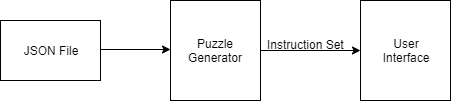
\includegraphics[scale=0.7]{Diagrams/Puzzle_System_Instruction_Flow.png}
\end{figure}

The JSON file associated to the puzzle level also tells the user interface which
instructions were left in the editor (Figure \ref{fig:Instruction_Flow2}). The intial state of the puzzle level leaves the
editor empty. Otherwise, the editor is populated with the same instructions that were
left during a previous attempt. This also includes final solutions that actually solved the
puzzle level.

\begin{figure}[!hb]
  \caption{Loading Instruction Editor State}
  \label{fig:Instruction_Flow2}
  \centering
  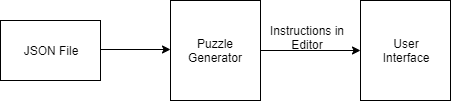
\includegraphics[scale=0.7]{Diagrams/Puzzle_System_Instruction_Flow2.png}
\end{figure}

\newpage

\subsection{User Interface System}
The User Interface will be one of the most important aspects of \textit{Computron}. 
The UI will represent the player's primary mode of interaction with the game. In 
addition, the UI will be the main source of text-based information for the player. An 
overview of the major components of the UI can be seen in Figure \ref{fig:ui_sytem_diagram}.\\

\begin{figure}[!hb]
    \caption{UI System Overview}
    \label{fig:ui_sytem_diagram}
    \centering
    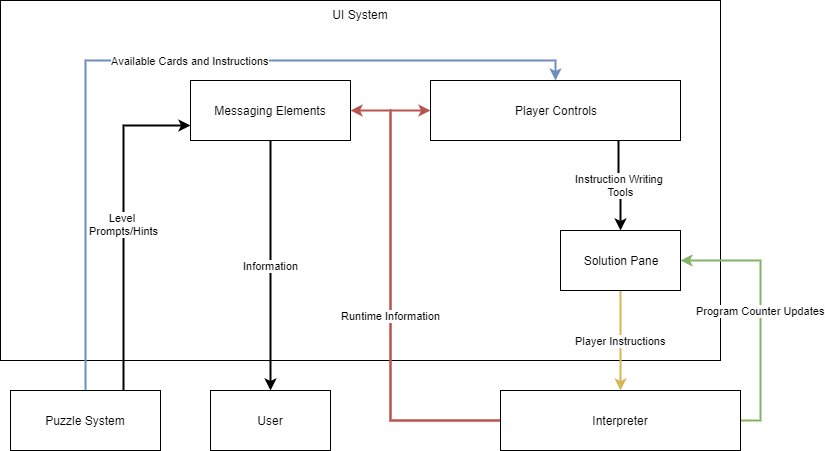
\includegraphics[width=\textwidth]{Diagrams/UI_Overview.png}
\end{figure}

\subsubsection{Player Controls}
As the player engages with the game, they will be able to control the simulation of 
their solution as it is executed in the puzzle game space. Once the player is ready to 
test out a solution, they will press a button to begin execution. At this point, the 
Interpreter will get the instructions from the UI and determine the sequence of steps 
that will simulate the solution. This gets communicated to the Actor to determine the 
moves it will take across the game space. As the Actor progresses through its actions, 
it communicates with the UI to grab data from UI elements and move data to other UI 
elements. These simulation steps cannot just be discarded once they are completed, 
since the player has controls to pause the simulation, proceed, or rewind to previous 
steps. These player controls will require the UI to communicate with the Actor, so that 
the Actor knows if it should continue with the next action, stop, or rewind the previous 
action.\\

\subsubsection{Solution Pane}
The solution pane is where the player must utilize available instructions to construct a 
solution to the current puzzle. The set of available instructions is received from the 
puzzle system to the UI. When the player is ready to execute their solution, the sequence 
of instruction commands is sent to the interpreter to analyze and decide what actions will 
be taken. The location of this element in the puzzle scene can be seen in our unified 
prototype (Figure \ref{fig:Unified_Prototype}).\\

\subsubsection{Player Messaging}
Controlling the flow of information to the player presents both technical and design 
issues to the team. Providing too many hints, prompts, and explanations can quickly 
turn the game into a glorified textbook; however, providing too few will make the game 
feel frustrating and inaccessible to our target audience. The User Interface will be tasked 
with handling this complex problem space.   

For the UI to be capable of delivering relevant information to the player, it must communicate 
with other major game systems. The Puzzle System's data-driven approach will allow it to 
provide the UI with puzzle specific data for each level of the game. Hints, prompts, and 
descriptions to be displayed to the player can all be retrieved from the Puzzle System on 
level start-up. Removing the responsibility of managing what information to display will 
allow the UI Designer to focus on player controls, and regulating the flow of information 
to the player.\\

In addition to its interactions with the Puzzle System, the User Interface will also communicate 
with the Interpreter to capture and display runtime information to the player. Common 
communications include runtime errors, program counter updates, or messages to reflect 
conditions that arise during execution executing.\\
\newpage

\subsection{Interpreter System}
\subsection{Overview}
As the invisible interface between the player's instructions window and the Actor's 
execution logic, the Interpreter's responsibilities are considerably abstracted from 
normal gameplay programming. More specifically, the Interpreter is responsible for 
defining the game's assembly-like language, extracting player instructions from the 
user interface, and marshaling the release of commands to the actor for execution.\\

\subsubsection{Language}
In order to keep the game accessible to inexperienced users, we developed a simple
pseudo-language to manage the manipulation of the puzzles. Below are the 13 instructions that 
make up the CAL.

\begin{itemize}
 	\item INPUT\\
	The INPUT command instructs Computron to approach the puzzle's Input Box and 
	retrieve the next value. If Computron is currently holding a value, he will discard it. 
	If the Input Box is empty, Computron will retrieve and hold a NULL value.
	\item OUTPUT\\
	The OUTPUT command instructs Computron to approach the puzzle's Output Box 
	and deposit his current value. If Computron is not holding anything, this instruction 
	will be considered invalid and raise a runtime error. Otherwise Computron will deposit 
	the value in the output box.
	\item JUMP\\
	The plain JUMP command instructs the interpreter to unconditionally move the program 
	counter to a new line in the player's solution. This instruction has no effect on Computron.
	\item JUMP IF NULL\\
	The JUMP IF NULL is a conditional jump instruction, which is only activated if the Actor
	 is not holding any value. This instruction is often used to break out of loops.
	\item JUMP IF LESS [X]\\
	The JUMP IF LESS [X] is a conditional jump instruction, which is only activated if the 
	value the Actor is holding is less than the value stored in player-specified register X. If 
	register X is empty, this instruction will be considered invalid and raise a runtime error.
	\item JUMP IF GREATER [X]\\
	The JUMP IF GREATER [X] is a conditional jump instruction, which is only activated if 
	the value the Actor is holding is greater than the value stored in player-specified register 
	X. If register X is empty, this instruction will be considered invalid and raise a runtime error.
	\item JUMP IF EQUAL [X]\\
	The JUMP IF GREATER [X] is a conditional jump instruction, which is only activated if 
	the value the Actor is holding is greater than the value stored in player-specified register 
	X. If register X is empty, this instruction will be considered invalid and raise a runtime error.
	\item MOVETO [X]\\
	The MOVETO [X] command instructs Computron to move the value currently being 
	held into the player-specified register X. If Computron's hands are currently empty, this 
	instruction will be considered invalid and raise a runtime error. If there is a value currently in 
	the register, it will be overwritten.
	\item MOVEFROM [X]\\
	The MOVEFROM [X] command instructs Computron to remove the value currently being 
	stored in the player-specified register X. If the register is empty, Computron will retrieve 
	and hold a NULL value. If Computron is currently holding a value, it will be overwritten.
	\item COPYTO [X]\\
	The COPYTO [X] command instructs Computron to move the value currently being held 
	into the player-specified register X. Computron will retain a copy of the number. If 
	Computron's hands are currently empty, this instruction will be considered invalid and raise a 
	runtime error. If there is a value currently in the register, it will be overwritten.
	\item COPYFROM [X]\\
	The COPYFROM [X] command instructs Computron to retrieve a copy of the value currently 
	being stored in in the player-specified register X. If the register is empty, Computron will 
	retrieve and hold a NULL value. If Computron is currently holding a value, it will be overwritten.
	\item ADD [X]\\
	The ADD [X] command instructs Computron to add the value stored in player-specified 
	register X to the value currently held. If either Computron's hands or register X are empty, this 
	instruction will be considered invalid and raise a runtime error. Otherwise, Computron will 
	perform the addition and overwrite his current value.\\
	\item SUBTRACT [X]\\
	The SUBTRACT [X] command instructs Computron to subtract the value stored in 
	player-specified register X from the value currently held. If either Computron's hands or 
	register X are empty, this instruction will be considered invalid and raise a runtime error. 
	Otherwise, Computron will perform the subtraction and overwrite his current value.
\end{itemize}

\subsubsection{Program Counter}
To facilitate proper simulation of the player's solution, the interpreter will need to maintain 
a program counter that iterates and jumps through the player's code appropriately. To 
ensure that these updates happen correctly, the Interpreter will need to rely on reports 
from the Actor that state the validity of instructions and the result of conditional expressions.
Updates to the program counter are forwarded to the Puzzle's UI system to maintain a 
visual representation of the program counter while the solution executes.

\subsubsection{UI Interface}
In addition to updating the program counter, the Interpreter is closely tied to the Puzzle UI's primary
control panel. The Start, Step, and Halt buttons all tie directly to the Interpreter's control interface.
Figure \ref{fig:interpreter_UI_interface} illustrates the nature of these interactions.

\begin{figure}[!htb]
	\caption{Interpreter/UI Interface Overview}
	\label{fig:interpreter_UI_interface}
	\centering
	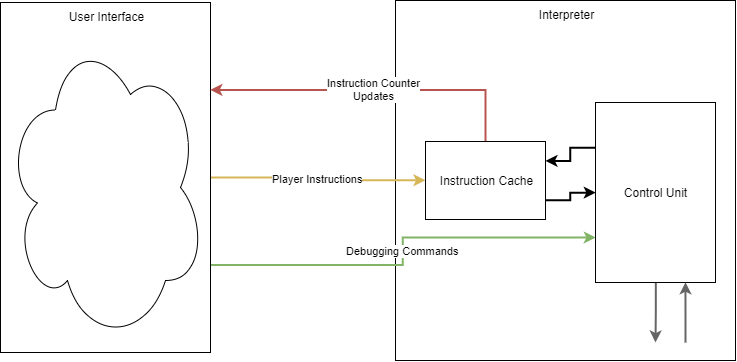
\includegraphics[width=\textwidth]{Diagrams/Interpreter_UI_Interface.png}
\end{figure}

\subsubsection{Actor Interface}
The Interpreter's Actor interface is responsible for making instructions available to the 
Actor on demand. In order to ensure the program counter is updated properly, the 
Interpreter and Actor engage in a three part handshake, shown in 
\ref{fig:interpreter_Actor_interface}.\\

\begin{figure}[!hb]
    \caption{Interpreter/UI Interface Overview}
    \label{fig:interpreter_Actor_interface}
    \centering
    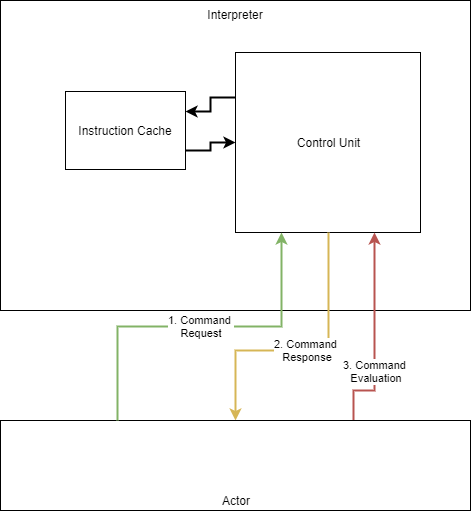
\includegraphics[width=\textwidth]{Diagrams/Interpreter_Actor_Interface.png}
\end{figure}

\newpage
The stages of the handshake are:
\begin{enumerate}
	\item Command Request\\
	The first step of the Actor control exchange is the Command Request. The Actor 
	will issue a Command Request to the Interpreter when the next player instruction is needed.
	\item Command Response\\
	The second step of the exchange is the Command Response. This response will be a 
	data structure for the actor to parse, including the next instruction's opcode and argument.
	\item Command Evaluation\\
	The last step of the exchange is the Command Evaluation. This stage is the Actor's chance 
	to report runtime errors to the Interpreter if the instruction is deemed invalid and report 
	the result of a conditional expression if the instruction included one. 
\end{enumerate}

\subsubsection{CAL Virtual Machine}
The Actor's implementation of the CAL is tightly coupled to the physical state of the puzzle. In addition,
it performs many non-executing tasks to visualize the language. These conditions made the unsuitable for 
conducting performance and correctness evaluations. To support those functions of solution grading the Interpreter
manages a Computron Assembly Language Virtual Machine (CALVM) object. The CALVM allows the interpreter to simulate
player solutions rapidly, and inspect runtime data like error states and cycle count easily. 
\newpage

\subsection{Actor System}
\subsubsection{Overview}
The Actor will be responsible for simulating the execution of the solution constructed
by the player through movement and animations. It is an animated character in the game that will move around the Puzzle Scene and manipulate the data elements of the current puzzle based on the sequence of commands that the player constructs in the Solution Pane of the User Interface. \\

Figure \ref{fig:actor_diagram} provides a high-level outline of the Actor component, all of its internal processes, and how it interacts with the other core aspects of the game.\\

\begin{figure}[!htb]
  \caption{Actor Component Overview}
  \label{fig:actor_diagram}
  \centering
  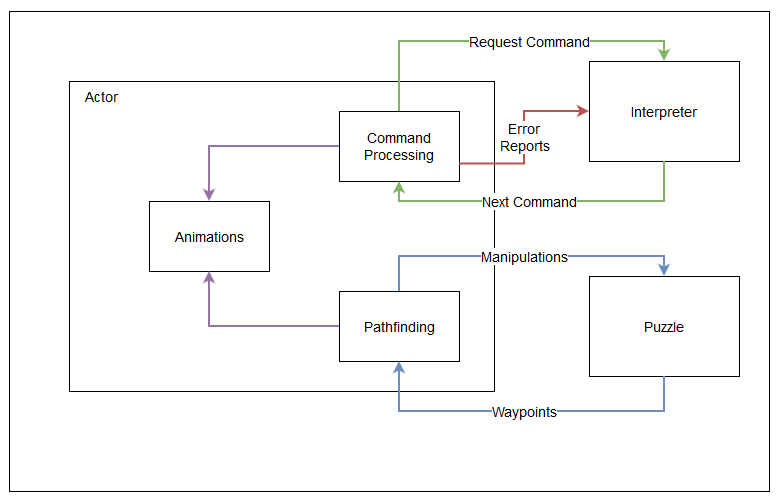
\includegraphics[scale=0.8]{Diagrams/actor_diagram.png}
\end{figure}
\newpage
The responsibilities of the Actor are as follows:

\begin{itemize}
	\item Retrieve commands from the Interpreter component
	\item Alert the Interpreter component to halt execution when an invalid command is attempted
	\item Move to the correct waypoints based on the command received
	\item Properly handle data manipulation in the puzzle scene (move and update data elements
			as specified by the current command)
	\item Communicate the flow of execution to the player through animations
	\item Illustrate to the player how data changes in response to commands via animations
	\item Act as a liason to the player for hints and other important messages.
\end{itemize}

\subsubsection{Interpreter Interactions}
Effective integration with the Interpreter is a key component of the functionality of the Actor. The Actor relies completely on the command sequence from the Interpreter in order to illustrate the execution of the solution. The Actor will continue to retrieve the next command in sequence from the Interpreter until the sequence terminates or an invalid command is attempted. If the command can be executed, the Actor will carry out the instruction visually so that the player can understand the flow of execution and the logic behind their solution. If the command causes an error in execution, the Actor will alert the Interpreter to halt execution. The flow of this process between the Actor and Interpreter can be seen in Figure \ref{fig:interpreter_interactions}.\\

\begin{figure}[!htb]
  \caption{Interactions between the Interpreter and Actor components}
  \label{fig:interpreter_interactions}
  \centering
  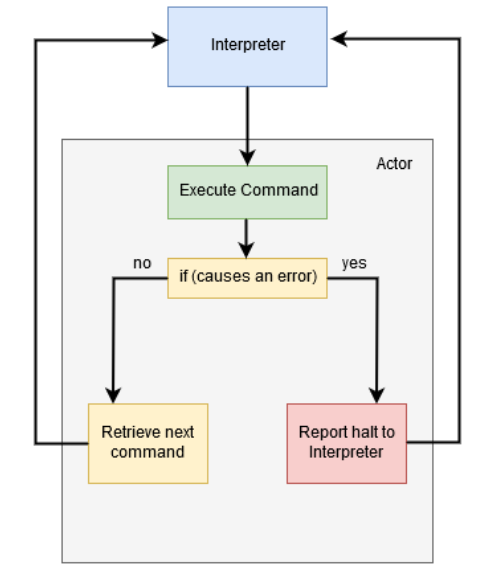
\includegraphics[scale=0.8]{Diagrams/interpreter_interactions.png}
\end{figure}

\subsubsection{Processing Commands}
The processing of commands is the core function of the Actor. Interfacing with the Interpreter component is only the first part of command processing; the majority of that processing occurs independently within the Actor component once a command has been retrieved. Figure \ref{fig:processing_commands} shows in detail how the Actor internally processes commands.\\

\begin{figure}[!htb]
  \caption{The state diagram followed by the actor when processing commands}
  \label{fig:processing_commands}
  \centering
  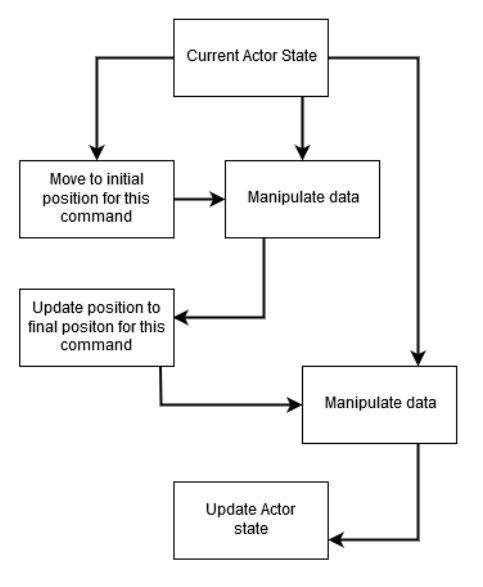
\includegraphics[scale=0.8]{Diagrams/processing_commands.png}
\end{figure}

After fetching a command, the Actor will then execute a series of movements and actions to carry out that command. This includes moving to the proper waypoint to initiate the instruction, manipulating data from the Puzzle Scene object the Actor is currently at, moving to a second waypoint to continue execution, and manipulating data at that second Puzzle Scene object. Depending on what the current command is and the status of the actor when the new command is retrieved, some of these four steps may not be applicable. Parsing each instruction separately and successfully regardless of the current state is vital. Commands that cause errors must be reported accurately back to the Interpreter so that execution can be halted when they are encountered, and no false reporting can be tolerated. If the command won't cause an error until it is partially completed, the partial execution of that command must be shown. Additionally, commands that can complete without causing errors should always be carried out exactly as specified. This is integral to the process of the game because even if the command is the wrong selection at the time, it still needs to be executed properly in the puzzle to show the player the error in their logic. Of course, correct commands that work towards the solution also need to be executed properly to eventually reach the solved state of the puzzle.\\

\subsubsection{Player Messaging}
The Actor is also the main form of direct communication with the player. Through the visual execution of the instructions that the player has selected, the Actor conveys how the solution the player built functions. This includes not just moving around the board and manipulating the data elements, but also providing visual cues to the user via detailed animations. For example, the data elements will be visibily picked up and held by the Actor. If that data is copied to another location, the Actor will be seen producing a copy of that data and placing it at the location specified. Data that is incremented or decremented via commands will be changed according to those commands so that the player sees and understands how the data elements are being manipulated. Additionally, providing expressive and emotive animations enhances the clarity of communication without bogging down the player with too much text. If the current command is to select the next element from Input but the Input box is empty, the Actor would attempt to pick up the item, find that nothing is there, and then emphasize that their hands are empty.\\

Aside from effective visual communication, the Actor will also provide information to the player via text when necessary. This form of communication will be used sparingly and will always be coupled with visual cues to help cut down on the amount of explicit text required to convey the information to the player. Because the Actor is essentially the only character in the game as well as the focus of the game action, any dynamic messaging that needs to occur will come from the Actor. Static messaging that does not change based on current activity will be left to the User Interface. Expanding on this idea of the Actor being a point of contact, if the player finds they are stuck on a certain puzzle they can click on the Actor in the field and request a hint on the solution for the current puzzle. \\
\newpage
\newpage

\section{Budget and Financing}
  There are no known budget or financing requirements at this time.\\
Current budget: \$0\\
Financing: \$0\\
Sponsorship: \$0\\

\newpage

\section{Milestones}
  This section of the document describes the major milestones of our project that we set
as regular interval goals for our success.

\subsection{Big Prototype Party (Monday, Oct 14th)}

\subsubsection*{Summary}
Since this project does not have a sponsor, the onus is on us to determine the
exact nature of the problem we would like to solve. To ensure that our efforts
are directed effectively for the remainder of our project, our first month has
been dedicated to researching and playtesting. By this date, every member of the
team should have a solid foundation of the problem space we are working in, and
have a prototype of a solution.

\subsubsection*{Deliverables}
Every member of the team must have a prototype of our final game. This prototype
should fit the following criteria:
\begin{itemize}
	\item The prototype is interactive.
	\item The prototype is engaging to work with.
	\item The prototype represents a wide slice of the game’s mechanics.
	\item The prototype makes the player think computationally.
	\item The rules of the prototype are concise and written out.
\end{itemize}

\subsection{Game Pitch (Friday, October 18th)}

\subsubsection*{Summary}
This milestone culminates one of the most critical stages of our project. Now
that we’ve had the time to demonstrate non-abstractly what our problem space is
and how we’d like to solve it, we can converge on a unified solution. By this
milestone the team should be able to confidently answer the following questions,
and develop the documentation necessary to capture our answers:
\begin{enumerate}
	\item What will our final product look like?
	\item What are the learning objectives of our game?
	\item What kind of puzzles will our game have?
	\item How will those puzzles work?
	\item How will those puzzles achieve our learning objectives?
	\item How will we order these puzzles to ensure that there is an appropriate
	learning curve?
	\item What evidence do we have that our learning curve will be engaging and
	effective for our target audience?
	\item What games did we draw inspiration from?
\end{enumerate}

\subsubsection*{Deliverables}
This milestone’s deliverables are still non-code items. These are items that we
will rely on for the remainder of our project, and inform all future efforts.
Specifically, we must deliver:
\begin{itemize}
	\item A unified prototype of our final game.
	\item A write up of our prototype, its capabilities, and its design philosophy.
	\item Diagrams/concept drawings of game mechanics not demonstrated by the prototype.
	\item Research Papers that support our design choices.
	\item Playtesting findings that support our design choices.
	\item Any other artifacts necessary to answer the questions above.
\end{itemize}

\subsection{Paper Prototype 2.0 (Monday, October 28th)}

\subsubsection*{Summary}
Rapid iteration is an important part of successfully designing a game. By this
milestone, our original prototype should be placed in the hands of as many
playtesters as possible. The group should use the data from this playtesting to
inform any design changes we make to our prototype.

\subsubsection*{Deliverables}
\begin{itemize}
	\item A new prototype of our final game, with documentation supporting our
	changes to our original prototype.
	\item Expanded design documentation to capture the vision of our final game
	including:
	\begin{itemize}
		\item Detailed system diagrams that describe how the mechanics of our game
		interact.
		\item An explanation of who will be the lead on certain areas of our game.
	\end{itemize}
\end{itemize}

\subsection{Hello Game (Friday, Dec 13th)}

\subsubsection*{Summary}
This milestone marks our the delivery of our proof of concept prototype. The teams' 
advisor will evaluate the prototype and provide recommendations for moving forward. 
The prototype will show an extremely basic vertical slice of our final game. 

\subsubsection*{Deliverables}
The only deliverable for this milestone will be the Hello World prototype. This prototype 
should meet the following requirements:
\newpage
\begin{itemize}
	\item Usability\\
	The prototype shall show the entire scene flow of our game. A user should be 
	able to move between the Main Menu, Puzzle Selection, and Puzzle Scenes at will. 
	The game should respond to these requests gracefully, and never leave the user 
	trapped in a scene. 
	\item Game Mechanics\\
	The foundations of the game's major mechanics should be in place and interactable. 
	The expected functionalities of the demo are specified below by scene.
	\begin{itemize}
		\item Main Menu\\
		The Main Menu scene should display the game's working title, \textit{Computron}, 
		as well as a functional play button that will bring the user to the Puzzle Selection 
		Scene. The scene should also have a placeholder background image.
		\item Puzzle Selection Scene\\
		The Puzzle Selection Scene should display a placeholder level graph, with selectable 
		nodes. Each node should transfer the player to the Puzzle Scene. The player should 
		also be able to return to the main menu.
		\begin{figure}[!hb]
			\begin{center}
			\caption{Sample level graph}
			\label{fig:boat1}
			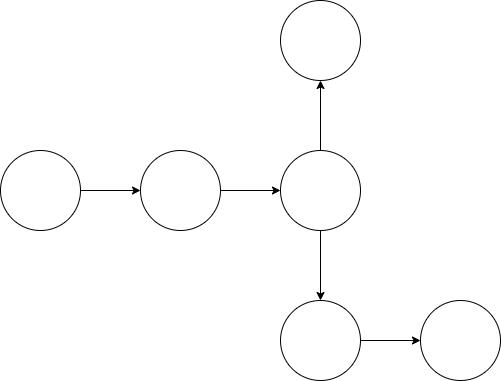
\includegraphics[width=5cm]{HelloWorldLevelSelect.png}
			\end{center}
		\end{figure}
		\item Puzzle Scene\\
		The Puzzle Scene will be the most involved portion of our prototype. Desired 
		mechanics are listed below by discipline:\\

		\textbf{UI:} The Puzzle UI will need to allow the player to perform the basic 
		puzzle solving operations. It should present the player with an instruction 
		set (\textit{Input, Output}) from which they may drag instructions into a solution 
		window. The Puzzle UI should present controls to allow the player to begin and 
		terminate the simulation of their solution. When the player's solution is being executed, 
		the UI should prohibit alterations to the solution window and display a program 
		counter to mark the current instruction being executed.\\

		\textbf{Level Design:} The level design of the Puzzle Scene will present all of the 
		static elements that will be present in every puzzle of our game. It will display an 
		input box with randomly generated contents, an output box that can accept objects 
		from the Actor, and a simple background plate.\\

		\textbf{Puzzle Logic:} Working in tandem with the level design, the puzzle scene's 
		logic system should be operational. Puzzle Logic is responsible for loading the scene 
		with the appropriate puzzle information. This includes a randomly generated input 
		box, the level prompt, an expected output, and the logic to read the output box 
		upon program completion to grade the player's solution.\\
    
		\textbf{Interpreter:} The Interpreter is the glue that binds the UI controls to the 
		Actor system. For this milestone, the Interpreter should be able to access and 
		process the player's solution stored in the solution window. When the player 
		starts the simulation, the Interpreter should process the instructions (ensuring 
		none are malformed) and make them available to the Actor upon request. 
		When the Actor requests an instruction, the interpreter will update its program 
		counter accordingly and report the counter's new position to the UI. The 
		Interpreter's PC calculation should be fully operational for the Input, Output, 
		and Unconditional Jump commands.\\

		\textbf{Actor:} For this milestone, the Actor should be able to query the Interpreter 
		for instructions to execute and interact with static level elements. Upon receiving an 
		input command, the Actor should move to the input box and remove at item. The 
		currently held item should be displayed on the Actor. Upon receiving an output 
		command, the Actor should move to the output box and deposit the currently 
		held item. If the Actor does not have an item in hand, it should report a fault to the 
		Interpreter so that simulation can be halted. If the Actor sees two input commands 
		back to back, it should discard its currently held item and attempt to take from the 
		input box again.\\
	\end{itemize}
\newpage
	\item Art\\
	For this milestone, programmer art placeholders are acceptable. However, the team should 
	have a plan in place to acquire quality art assets.
\end{itemize}

\subsection{Waterfall Method (Thursday, December 5th)}

\subsubsection*{Summary}
This milestone marks the deadline for Senior Design I documentation submission. This document 
must be complete, professionally bound, and delivered to HEC-345 by 1:00PM.

\subsubsection*{Deliverables}
As per the requirements of this course, our final design document will describe
all aspects of the project including:
\begin{enumerate}
	\item An Executive Summary\\
	The Executive Summary will give a high level overview about the purpose of the project 
	and how the project will fulfill that purpose. The Executive Summary should be written in 
	language accessible to non-technical professionals.
	\item A section detailing project significance\\
	This section should echo our Executive Summary in greater detail, with more specific language.
	\item A section describing our requirements\\
	This section should include an exhaustive list of our project's functional and non-functional requirements.
	\item A section detailing our game's design process\\
	This section should describe the team's efforts in discovering project requirements, and relate 
	the game mechanics chosen to the projects goals.
	\item A section detailing our game's technical design\\
	This section should describe the layout of the game's code systems. It should include 
	detailed technical discussions and diagrams to guide development.
	\item The project's milestones\\
	The milestones will be sets of requirements to ensure the project remains on track.
\end{enumerate}

\subsection{Open to Interpretation (Friday, January 10th)}

\subsubsection*{Summary}
``Open to Interpretation" will mark the project's first Alpha release. In this state, the game 
should be functional enough to place in front of a playtester with minor developer 
intervention. All basic game mechanics will be fully functional, and observing gameplay 
should produce relevant observations for the development team.

\subsubsection*{Deliverables}
This milestone’s deliverable is a stable Alpha release of our game. The requirements of the 
Alpha release are as follows:

\begin{itemize}
	\item Player experience\\
	The player experience should be polished enough to allow an individual with no 
	experience with our project to pick up and play it. All controls presented to the 
	player should work as expected, free of any noticeable bugs or glitches. Menus 
	should allow for proper flow between the game's scenes, and incomplete or 
	non-functional menus should be marked as such.

	Specifically, the player should be able to perform the following operations:
	\begin{enumerate}
		\item Launch the game from outside the Unity Editor.
		\item Start the game from the main menu, and enter the puzzle selection scene.
		\item Upon first run, only the first level of the game should be unlocked.
		\item Subsequent levels will only be unlocked after the player completes a puzzle.
		\begin{itemize}
			\item Exiting a puzzle without solving it will not unlock new puzzles
		\end{itemize}
		\item Puzzle unlocking will have an associated visual when returning to the level select screen.
		\begin{itemize}
			\item Player controls will be disabled and player focus should be drawn to the unlocked levels. (e.g. Camera zoom, simple animations, etc.)
		\end{itemize}
		\item After selecting a puzzle, the player should be transferred to the puzzle scene. The game should have at least two distinct levels.
		\item In the puzzle scene, the following mechanics should be operational.
		\begin{itemize}
			\item The instruction set pane shows only the subset of instructions chosen 
			to be available for that puzzle.
			\item Instructions can be dropped into the solution pane and manipulated in an intuitive way
			\item If the puzzle includes Memory Cards, the cards are displayed at the 
			bottom of the screen and are interactable.
			\item Move and Copy instructions are not usable until at least one 
			Memory card is in play.
			\item Memory Cards can be placed on, removed from, and re-ordered in 
			the play area.
			\item A Memory Card cannot be removed if it is referenced by an 
			instruction in the solution window. Instructions blocking card removal are 
			highlighted when the player's request fails.
			\item Computron is capable of interacting with the Inbox, Outbox, and registers.
		\end{itemize}
	\end{enumerate}
	\item Available Puzzles\\
	Puzzles 3, 4 of the tutorial sequence specified in Section~\textbf{\ref{section:tutorial}}.
	\item Available Mechanics
	\begin{itemize}
		\item Level Selection\\
		The level selection scene allows players to chose which puzzle they'd like to attempt. 
		Choosing a level should transfer the player to the Puzzle Scene with the relevant puzzle 
		data loaded. The player will be restricted in which puzzles are available, and have more unlocked as they successfully complete them.
		\item Basic instruction writing\\
		Player can click and drag the INPUT, OUTPUT, MOVETO, MOVEFROM, JUMP, and 
		JUMP IF NULL instructions into the instruction pane. Jump instructions allow player 
		to click-and-drag to set jump anchor.
		\item Basic Memory Card Manipulation\\
		Player is presented and can interact with a hand of memory cards on levels that require 
		them. Cards can be played, reorganized, and removed. MOVETO and MOVEFROM 
		instructions are active if and only if there is at least one Memory Card on the board.
		\item Basic Solution Grading\\
		After a player completes a puzzle, they are presented with a score sheet that provides 
		metrics on the par for:
		\begin{itemize}
			\item Instruction count
			\item Solution Runtime
			\item Memory Card cost
		\end{itemize}
		After they are done viewing this screen, they will be transferred back to the puzzle selection scene where they will see new levels unlock.
	\end{itemize}
\end{itemize}

\subsection{Tutorializing (Wednesday, February 12th)}

\subsubsection*{Summary}
``Tutorializing" will mark the Computron's second Alpha release. For this release, the tutorial 
system will be greatly expanded to allow for more hands-off playtesting.

\subsubsection*{Deliverables}
This milestone’s deliverable is another stable Alpha release of our game. The expected new 
features are listed below:

\begin{itemize}
	\item Available Puzzles\\
	Puzzles 1 through 9 of the tutorial sequence specified in Section~\textbf{\ref{section:tutorial}}.
	\item Available Mechanics
	\begin{itemize}
		\item Level Selection\\
		The level selection menu should meet the following requirements:
		\begin{itemize}
			\item Level selection menu supports a strong ordering of tutorial levels.
			\item Level selection menu allows for optional paths that do not impede player 
			progression
			\item The player's performance on puzzles (number of stars) should be recorded 
			and restored between play sessions.
			\item Advanced levels should be restricted from play until the player earns the 
			requisite number of points to unlock them.
		\end{itemize}
		\item Instruction Writing\\
		The puzzle writing and interpreting system should support the following instructions:
		\begin{itemize}
			\item INPUT
			\item OUTPUT
			\item JUMP
			\item JUMP IF NULL
			\item JUMP IF LESS
			\item JUMP IF GREATER
			\item MOVETO X
			\item MOVEFROM x
		\end{itemize}
		\item Memory Card Manipulation\\
		Player memory card interactions should be well polished. Players should find 
		playing and removing cards an intuitive part of the puzzle solving process. In 
		addition, the following cards should be operational:
		\begin{itemize}
			\item Register
			\item Stack
		\end{itemize}
	\end{itemize}
\end{itemize}

\subsection{Breaking Beta (Friday, February 28th)}

\subsubsection*{Summary}
``Breaking Beta" is Computron's first Beta release. At this point, the game's minimum 
viable product should be feature complete, leaving ample time to rework and refine 
mechanics based on intense playtesting.

\subsubsection*{Deliverables}
\begin{itemize}
	\item Available Puzzles\\
	Puzzles 1 through 12 of the tutorial sequence specified in Section~\textbf{\ref{section:tutorial}}.
	\item Available Mechanics
	\begin{itemize}
		\item Instruction Introductions\\
		Messaging should be added to attract the player's attention to new instructions 
		when they are made available. Upon first receipt of a new instruction, the User 
		Interface should display an interactive menu that allows players to unbox their 
		new command.
		\item Instruction Writing\\
		In game documentation of how instructions work is available from the puzzle scene.
		\item Memory Card Manipulation\\
		In game documentation of how a memory card works is available from the puzzle scene.
	\end{itemize}
\end{itemize}

\subsection{FIEA Playtest (Monday, March 2nd)}

\subsubsection*{Summary}
The team's advisor has offered to allow \textit{Computron} to be playtested by students 
at the Florida Interactive Entertainment Academy (FIEA). Playtesters from FIEA will span 
both technical and non-technical roles in game development, and will be able to offer 
valuable insights. It will be imperative to capture these insights, and use them to guide the 
final stages of the game's development.

\subsubsection*{Deliverables}
For this playtest, the team should be able to present a high quality build of the game. 
Fielding a high quality demo will be very important in allowing the team to gather effective 
observations from the playtesters. The team should arrive to the playtest with:
\begin{enumerate}
	\item A stable build of the game.
	\item A set of exit survey questions to track player experience.
	\item Several computers capable of playing the game to allow increased playtesting 
	bandwidth.
\end{enumerate}

After the playtest, the team should compile player feedback and evaluate which parts 
of the game will need more attention.

\subsection{Quick Math (Friday, March 20th)}

\subsubsection*{Summary}
``Quick Math" will be the second Beta release of Computron. It will feature an expanded 
instruction set and new puzzles that make use of mathematical principles. 

\subsubsection*{Deliverables}
\begin{itemize}
	\item New Instructions\\
	Computron should support four brand new instructions:
	\begin{itemize}
		\item ADD X
		\item SUBTRACT X
		\item BUMP++
		\item BUMP-\--
	\end{itemize}
	\item New Puzzles\\
	This release should feature three new puzzles that exercise the new problem spaces 
	made accessible by the expanded instruction set:
	\begin{enumerate}
	\item Adding Machine\\
	This puzzle should introduce players to the mechanics of the new ADD instruction. 
	Puzzle should ask players to add pairs of numbers in the input and output their sum.
	\item Subractinator\\
	This puzzle should introduce players to the mechanics of the new SUBTRACT instruction. 
	Puzzle should ask players to subtract pairs of numbers in the input and output their difference.
	\item Hexiplier\\
	This puzzle should show players an application of the new ADD instruction. For each number 
	in the input, the puzzle should expect that number times 6 as output.
	\end{enumerate}
\end{itemize}

\subsection{Release Candidate (Friday, April 10th)}

\subsubsection*{Summary}
Nearing the end of our project, milestone requirements will largely be determined by 
the state of the game and the results of playtests. For this milestone, the team should 
have most of the concerns raised from the FIEA playtest fully remedied.

\subsubsection*{Deliverables}
A fun release candidate of \textit{Computron}.

\subsection{Mission Accomplished (Wednesday, April 15th)}

\subsubsection*{Summary}
``Mission Accomplished" marks the final release of \textit{Computron}. The project should 
be in a state that accomplishes the goals set forth in this document.

\subsubsection*{Deliverables}
A game the team is proud of.
\newpage

\section{Project Summary and Conclusion}
  \subsection{Summary}
The early stages of our project mainly consisted of research and testing. When we first began, we knew the main idea of our project -- an educational video game that taught players computer science concepts -- but we didn't have a clear definition on how that idea would be realized or the steps we needed to take to get there. We knew we didn't want to jump into designing the game and its mechanics without a clearly defined plan and endpoint in mind. As a team we combined efforts in researching and brainstorming to determine a general concept that our game would be based around. With a central idea defined, we each developed a paper prototype mock-up of what our version of the game would be and playtested it on people inexperienced with programming. The unified prototype was borne of our combined efforts and the information gathered from this initial research and development phase of \textit{Computron}.\\

After the unified prototype was formed, we each produced an identical whiteboard version of the game and tested it on as many people as we could. The testing went exceptionally well and we all agreed that we were ready to move forward with coding the game systems and mechanics. With a clear picture now forming as we began laying down the skeleton code to instantiate the basic layout of our game, we continued to fine tune the definitions and expectations of each aspect of our game and what the end result product should look like. This consisted not just of the physical appearance and feel of the game, but also the functionality of each component and how it should interact with other core components of the game. Additionally, the progression of puzzles that was designed for use with the prototype tested so well that it was adopted directly as the tutorial sequence for \textit{Computron}. Minor changes and additional levels were later added to the sequence, but the progression was found to be extremely effective.\\

Through frequent playtesting, we were able to refine a comprehensive design of our game. Working to implement key features was a driving focus, and informed the priority of minor features and supporting functionality. As a team, we strove to continuously keep our end goal in mind, and always maintained the priority of each sprint to reflect the end goal of the project as a whole. Through this focus and determination, we are able to now deliver an exhaustive and satisfying first pass at \textit{Computron}.\\

\subsection{Future Considerations}
We realize that six months is an incredibly tight turnaround time for a fully realized video game project, and are well aware that there is potential for improvement and iteration on our final version of \textit{Computron}. It is our dearest hope that future students will take interest in the groundwork we have laid here and aspire to expand upon the current offerings and capabilities offered herein. To this end, we would like to present a summary of possible improvements to guide others towards success in their efforts.

As it currently stands, \textit{Computron} has only a basic implementation of tutorial sequences implemented. We would like to see future iterations of the project expand upon the number of provided tutorials. Keep in mind that a tutorial punctuating every level of the main path becomes more annoying than helpful, so it would also be beneficial to ensure there are enough buffer levels between newly introduced instructions or cards, and thus, tutorials. The frequency of introducing new game elements and interrupting the player to deliver instructions versus the progression of puzzles and challenge presented in solving each one is a delicate balance, and requires extensive testing and refinement. Proceed with caution.\\

In addition to expanding the tutorials available to players, it would behoove the next team to adopt this project to refine the tutorial construction system to be more user friendly. As it stands now, building a tutorial is a fairly involved process. In order to enable the streamlining of expansion on \textit{Computron} in any further iterations, it is integral to construct a tutorial building system that is intuitive and effortless. By streamlining this process, we can collectively open up the possibility of introducing \textit{Computron} as course software and allow professors to customize the puzzles provided to fit course materials.\\

In the same sense, it could be beneficial to the application of \textit{Computron} to lend greater support to WebGL builds from Unity. In its current state, the game experiences some scaling errors based on monitor resolution and whether or not the user is in full-screen mode. As we are currently only set to support deployment to an independent desktop build for the main three operating systems, including better web deployment stability could be largely beneficial. In addition to web-based access, a system that implements a database to keep track of leaderboard scores could be used in conjuction with Introduction to Programming classes in order to not only provide students with an incentive to practice programming concepts, but also to allow professors to track the progress of students enrolled in their courses. This insight could help lecturers focus on topics students struggle with and allow them to spend less time on topics that students handle well.\\

Additionally, there are some minor tweaks that could be made to enhance the player experience. First, the visuals of the game have some room for improvement. Currently there are animations missing on the Computron character. The artists we had on board were able to get sprite sheets into the game for animations but they were not implemented because the art style of the character and the puzzle scene contrasted. They were in the process of collaborating to transfer the sprite sheets to the puzzle scene art style, but unfortunately did not make it into the build in time. Also, in game objects like data cubes are extremely basic and could be much more impactful with a bit of polish. Second, more levels and card awarding can go a long way to improve player investment in \textit{Computron}. Currently, only newly acquired instructions are being distributed via the awarding system. Expanding this to include cards would be immensely beneficial to players in conjuction with the expanded tutorial system. More levels in the progression sequence could help space the time between tutorials -- as previously mentioned -- as well as increase the incentive for players to continue practicing their computational thinking skills. A complementary feature of this would be including tooltips on each instruction type and card type to remind players of the description of an element whenever it is appropriate to do so (e.g., on right click, double left click, etc.). Furthermore, future developers might aspire to construct a  “card book" in the image of a card collector, where each card has an assigned slot in the book, and players can look through it at their leisure and review important information about each game element.\\

Some possible  “nice to have" features for future iterations of \textit{Computron} might include deeply clever star requirements, allowing multiple solutions to be saved for each puzzle, and the opportunity to submit more efficient solutions to the developers. For current star requirements, players are simply measured against the metrics for the best solutions that the developers could come up. It would be nice for future teams to revisit those solutions and see if they can find more clever ways to get better ratings for the awards metrics. Similarly, if a player happens to get a better score than the metrics set so far, it would be beneficial to submit that solution to the development team so that the game could be updated to reflect a better solution. This would, of course, involve more iteration or explanation. Again, the idea of an online leaderboard comes to mind for claiming and reporting solution efficiency. Additionally, some metrics of efficiency versus instruction count versus cycle count may not all be attainable on a single pass at a puzzle solution. It would be advantageous to allow users to solve multiple solutions for each puzzle in the game. This way, an optimally time efficient solution and an optimally space efficient solution could both be stored for future reference.\\

\subsection{Conclusion}
The extensive amount of research and playtesting that went into this project before development began was very informative of our design. Being able to change major components of the game without having to redesign or replace code was very beneficial, and we were able to develop a very clear idea of what we expected out of our project before we ever began implementing it. Running through our actual game on paper and being able to refine details that players found confusing or unintuitive helped shape the final vision of \textit{Computron} well ahead of the first line of code ever being written.\\

Minimizing the interactions between the four core systems of the game also helped us to reduce the spaces where problems might arise. Each major system of the game only communicates with two other systems, limiting the potential for errors to occur. While a considerable amount of work had to be done when building parts of the game that closely relied on interfacing with another system, we were largely able to work independently on our respective systems. This allowed a lot of progress to happen simultaneously and no one was ever left waiting for someone to finish something before they could work on their own system.\\

The early playtesting results have shown a lot of promise and positive feedback. Many players reported that the concept of the game is interesting and that the game is engaging to play. Most early constructive feedback was in response to systems that had not been fully completed, with some quality of life suggestions that have since been incorporated into our final design. With all major systems of the game in their current state, the majority of feedback revolved around polish requests for game visuals, with some suggestions for expansion on mechanics. These have been summarized in the Future Considerations section of this document. With that in mind, it is our opinion that this Computron 1.0 verision is an immense success as we were able to meet and exceed all of project goals.\\

\newpage

\section{References}
  %in the order that they appear in the document
[1] J. Cheon and K. Kwon. “Exploring problem decomposition and program
development through block-based programs”, In \textit{International Journal of
Computer Science Education in Schools}, April 2019\\

[2] D. Topalli and N. E. Cagiltay. "Improving programming skills in engineering 
education through problem-based game projects with Scratch", In 
\textit{Computers and Education}, 2018

[3] H. Liang et al. "Students' perception on the use of visual tilings to support their
learning of programming concepts", In \textit{International Conference on Teaching, 
Assessment and Learning for Engineering}, 2013

[4] L. Leifheit et al. “Programming Unplugged: An Evaluation of Game-Based
Methods for Teaching Computational Thinking in Primary School”, In
\textit{European Conference on Games Based Learning}, 2018
\newpage

\section{Appendices}
  \subsection{Appendix A}

\subsection{Appendix B}

\subsection{Appendix C}
\end{document}
